% don't remove the folling lines, and edit the defintion of \main if needed
\documentclass[../report.tex]{subfiles}
\providecommand{\main}{..}
\IfEq{\jobname}{\currfilebase}{\AtEndDocument{\biblio}}{}
\IfEq{\jobname}{\currfilebase}{%file for shortcuts

\newcommand{\nch}{\ensuremath{N_{\mathrm {ch}}\xspace}}
\newcommand{\Ncoll}{\ensuremath{N_{\mathrm {coll}}}}
\newcommand{\Npart}{\ensuremath{N_{\mathrm {part}}}}
\newcommand{\dNdeta}{\mathrm{d}N_\mathrm{ch}/\mathrm{d}\eta}
\newcommand{\snn}         {\ensuremath{\sqrt{s_{\mathrm {NN}}}}}
\newcommand{\kT}          {\ensuremath{k_{\mathrm {T}}}}

\newcommand{\pp}          {pp}
\newcommand{\pPb}         {pPb}
\newcommand{\pA}          {pA}
\newcommand{\PbPb}        {PbPb}
\newcommand{\AuAu}        {AuAu}
\newcommand{\CuCu}        {CuCu}
\newcommand{\pAu}         {pAu}
\newcommand{\dAu}         {dAu}
\newcommand{\lsim}        {\,{\buildrel < \over {_\sim}}\,}
\newcommand{\gsim}        {\,{\buildrel > \over {_\sim}}\,}
\newcommand{\co}[1]       {\relax}
\newcommand{\nl}          {\newline}
\newcommand{\el}          {\\\hline\\[-0.4cm]}}{}

\begin{document}

\section{Quarkonia}

\label{sec:quarkonia}

\textbf{Coordinators}: A. Andronic (M\"{u}nster University), E. Chapon (CERN)
\linebreak
\textbf{Contributors}: R. Rapp (Texas A\&M University), J.-P. Lansberg (Institut the Physique Nucl\'{e}aire d'Orsay), E. Ferreiro (Santiago de Compostela University)


%%%%%%%%%%%%%%%%%%%%%%%%%%%%%%%%%%%%%%%%%%%%%%%%%%%%%%%%%%%%%%%%
\subsection{Introduction}
\label{sec_intro}
%%%%%%%%%%%%%%%%%%%%%%%%%%%%%%%%%%%%%%%%%%%%%%%%%%%%%%%%%%%%%%%%
A key objective in high-energy heavy-ion physics is to determine the in-medium forces 
that give rise to the remarkable many-body features of the quark-gluon plasma (QGP).
In the QCD vacuum, the unravelling of the fundamental force between two static color charges  
was made possible by the discovery of the charmonium and bottomonium states in the 1970's. 
Subsequent quantitative analyses of the bound-state spectra established the underlying
potential to be of Cornell type~\cite{Eichten:1979ms}, 
\begin{equation}
V(r) = -\frac{4}{3} \frac{\alpha_s}{r} + \sigma r \ ,
\label{V}
\end{equation} 
with a colour-Coulomb term due to gluon exchange and a linear rising term with string
tension $\sigma\simeq0.9$\,GeV/fm. This potential has also been quantitatively confirmed 
by lattice-QCD (lQCD) simulations~\cite{Bali:2000gf}. 
The corresponding effective field theory of QCD, potential non-relativistic QCD
(pNRQCD), provides a rigorous framework for the description of the heavy quarkonium
bound-state spectra in the large-mass limit~\cite{Brambilla:2004wf}.
The heavy-quark (HQ) potential thus provides a well calibrated starting point to probe the 
QCD medium, and the in-medium spectroscopy of quarkonia is the natural tool to carry this 
out in heavy-ion collisions, cf.~\cite{Rapp:2008tf,BraunMunzinger:2009ih,Kluberg:2009wc,Mocsy:2013syh,Liu:2015izf} 
for recent reviews.
The string term in the HQ potential, eq.~(\ref{V}), characterizes the long-range nonperturbative 
part of the force and is associated with the confining property of QCD. It is expected to play 
a critical role in the transition from hadronic to partonic degrees of freedom, and may well be 
responsible for the remarkable transport properties of the QGP, {\it i.e.}, its strongly coupled 
nature, up to temperatures of 2-3 times the pseudo-critical temperature, $T_c$~\cite{Liu:2016ysz}. 

Much like in vacuum, a systematic investigation of the in-medium force must involve the 
{\em spectroscopy} of different states, as they subsequently dissolve with increasing 
temperature. In this sense, quarkonia are not straightforwardly usable as a thermometer, 
which would imply that their dissociation pattern provides a known gauge. In the vacuum, 
only the 1S ground-state bottomonia (\PGUP{1S} and \PGhb) are small enough in size 
to be mostly bound by the colour-Coulomb force. All excited bottomonia and all charmonia are 
predominantly bound by the nonperturbative string force (and/or residual mesonic forces). 
Thus, charmonia and excited bottomonia are excellent probes of the in-medium confining
force, as originally envisioned for the \PJgy~\cite{Matsui:1986dk}.
However, in the cooling of the expanding fireball, quarkonia can also be ``regenerated" 
through recombination of individual heavy quarks and anti-quarks diffusing through the medium. 
This mechanism has turned out to be critical in understanding the
\PJgy production systematics at the LHC where regeneration (or statistical hadronisation) 
constitutes the major part of the yield observed in central Pb-Pb collisions. It's precise
amount is sensitive to the open-charm cross section and the charm-quark diffusion
coefficient, whose determination are key objectives discussed in the chapter~\ref{sec:HI_HF} on open 
heavy-flavor production. For bottomonia, the current understanding suggests that regeneration 
is less 
important (although still significant) for \PGUP{1S}, but possibly figures as a
major component in the strongly suppressed yield of excited states, especially the 
\PGUP{2S}. It is therefore of great importance to obtain additional information about
the production "times" of the observed yields, in particular through $\pt$ spectra
and elliptic flow which contain information about the fireball's collectivity imprinted
on the quarkonia by the time of their decoupling. A schematic illustration of the current knowledge
extracted from ``in-medium quarkonium spectroscopy", {\it i.e.}, their production systematics 
in heavy-ion collisions is shown in Fig.~\ref{fig_pot}.        
\begin{figure}[!h]
\begin{center}
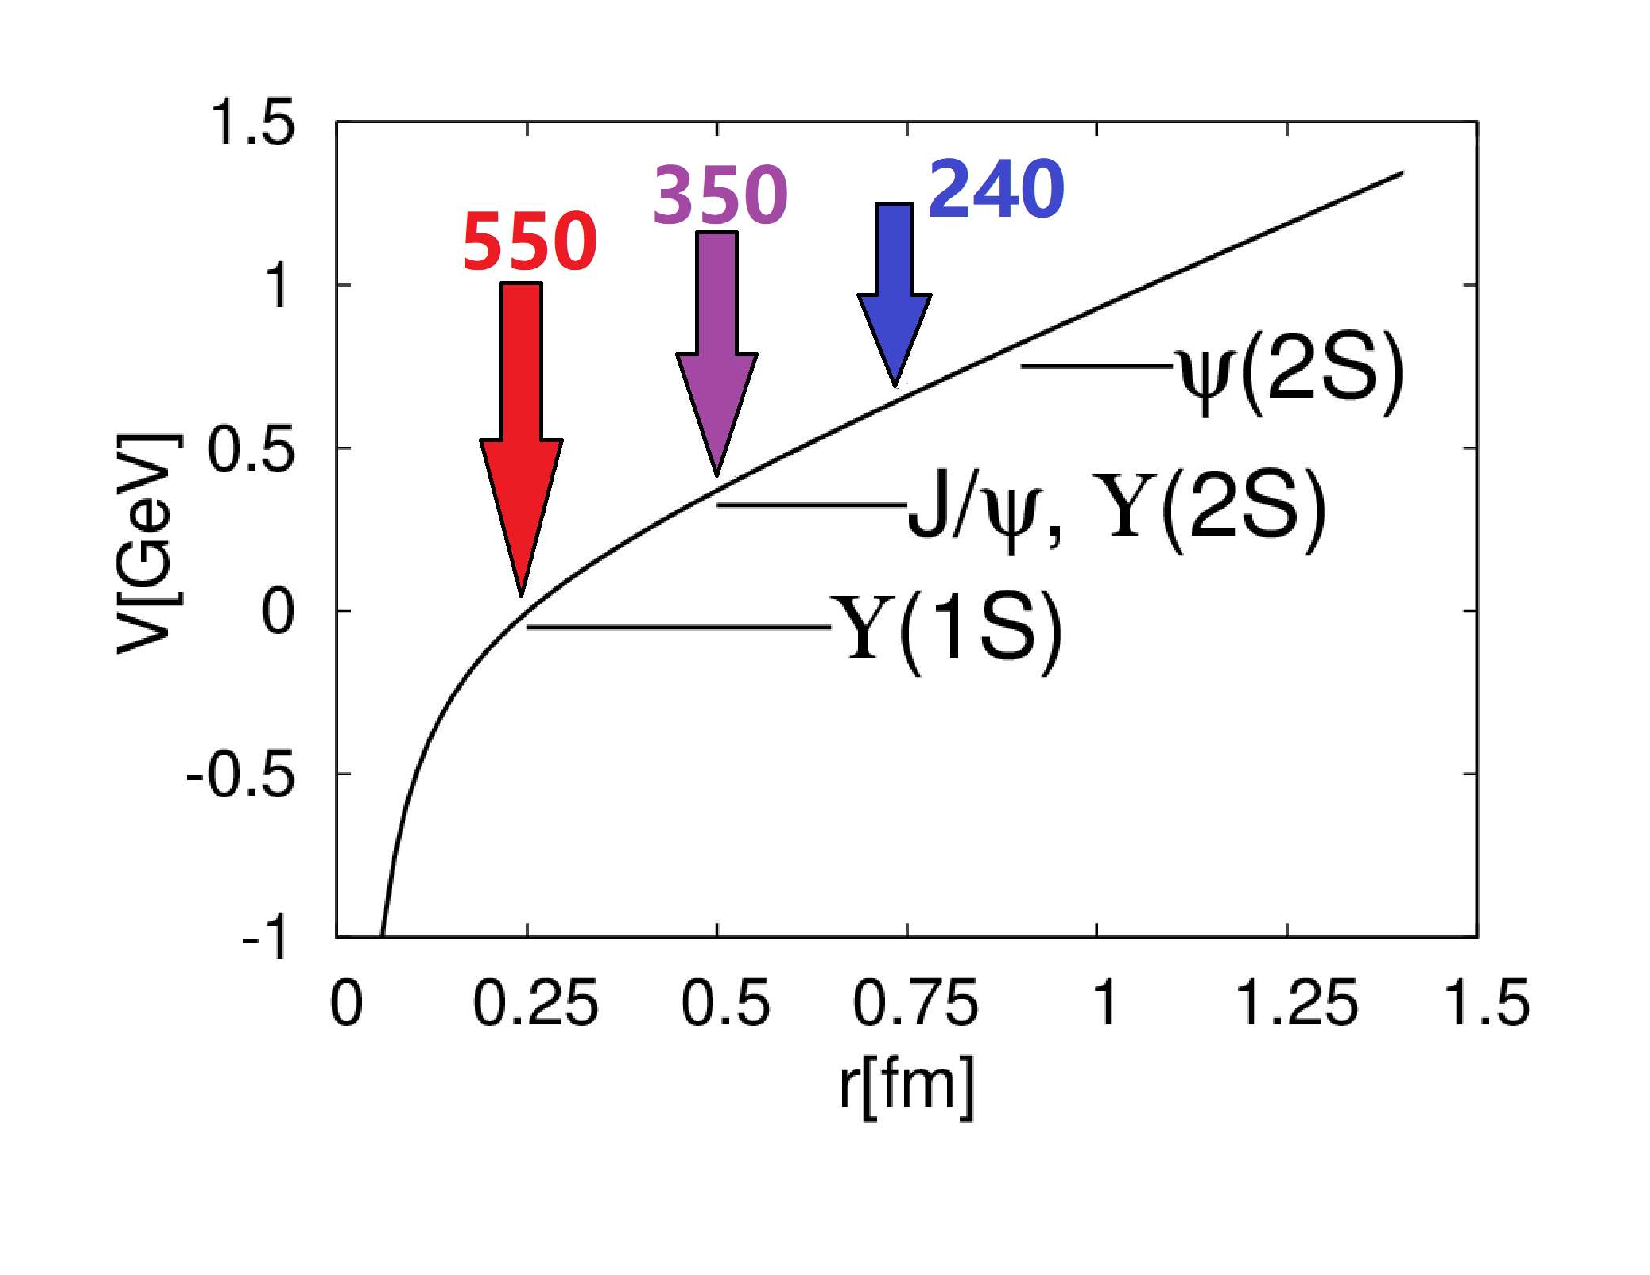
\includegraphics[width=0.6\columnwidth]{\main/quarkonia/fig/in-med-pot.pdf}
\end{center}
\vspace{-0.5cm}
\caption{The vacuum heavy-quark potential as a function of $Q\bar Q$ separation. The vertical
lines indicate the approximate locations of the vacuum bound states while the horizontal arrows
indicate the minimal screening distances of the media produced at the SPS, RHIC and LHC, as 
extracted from quarkonium production systematics in Pb-Pb and Au-Au collisions, along with 
approximate initial temperatures reached in these collisions. 
Figure taken from Ref.~\cite{Rapp:2017chc}}
\label{fig_pot}
\end{figure}


On the theoretical side, the basic objects are the quarkonium spectral functions which 
encode the information on the quarkonium binding energies, in-medium HQ masses and the
(inelastic) reaction rates. Ample constraints on the determination of the quarkonium
spectral functions are available from thermal lQCD, {\it e.g.}, in terms of the heavy-quark
free energy, euclidean and spatial quarkonium correlation functions, and HQ susceptibilities,
and are being implemented into potential model 
calculations~\cite{Wong:2004zr,Mocsy:2005qw,Alberico:2006vw,Brambilla:2008cx,Riek:2010py,Burnier:2015tda,Liu:2017qah}.
The information from the spectral functions can then be utilized in heavy-ion phenomenology
via transport models. As such, there is a rather direct connection between first-principles
information from lQCD and experiment that greatly benefits the extraction of robust information 
on the in-medium QCD force and its emergent transport properties (most notably the (chemical)
equilibration rates of quarkonia). 
Thus far most transport models are based on rate equations and/or
semiclassical Botlzmann equations. In recent years quantum transport approaches have 
received increased attention; it will be interesting to see how large the corrections
of these effects are to the semiclassical approaches. Quantum effects may be particular 
relevant at high $\pt$ in connection with the in-medium formation times of quarkonia, 
augmented by the Lorentz time dilation in the moving frame; schematic treatments of
this effect in semiclassical approaches suggest that varying formation times can leave 
observable differences for high-momentum charmonia and 
bottomonia~\cite{Song:2015bja,Hoelck:2016tqf,Du:2017qkv,Aronson:2017ymv,Krouppa:2017jlg}. 
Finally, the implementation of phase-space distributions of explicitly diffusing heavy quarks 
into quarkonium transport is being investigated by various groups, which, as mentioned above, 
will provide valuable constraints on the magnitude and \pt dependence of regeneration 
reactions.   

\subsection{Charmonia in PbPb collisions (Main contributor: Anton Andronic)}


\begin{figure}

\begin{center}
 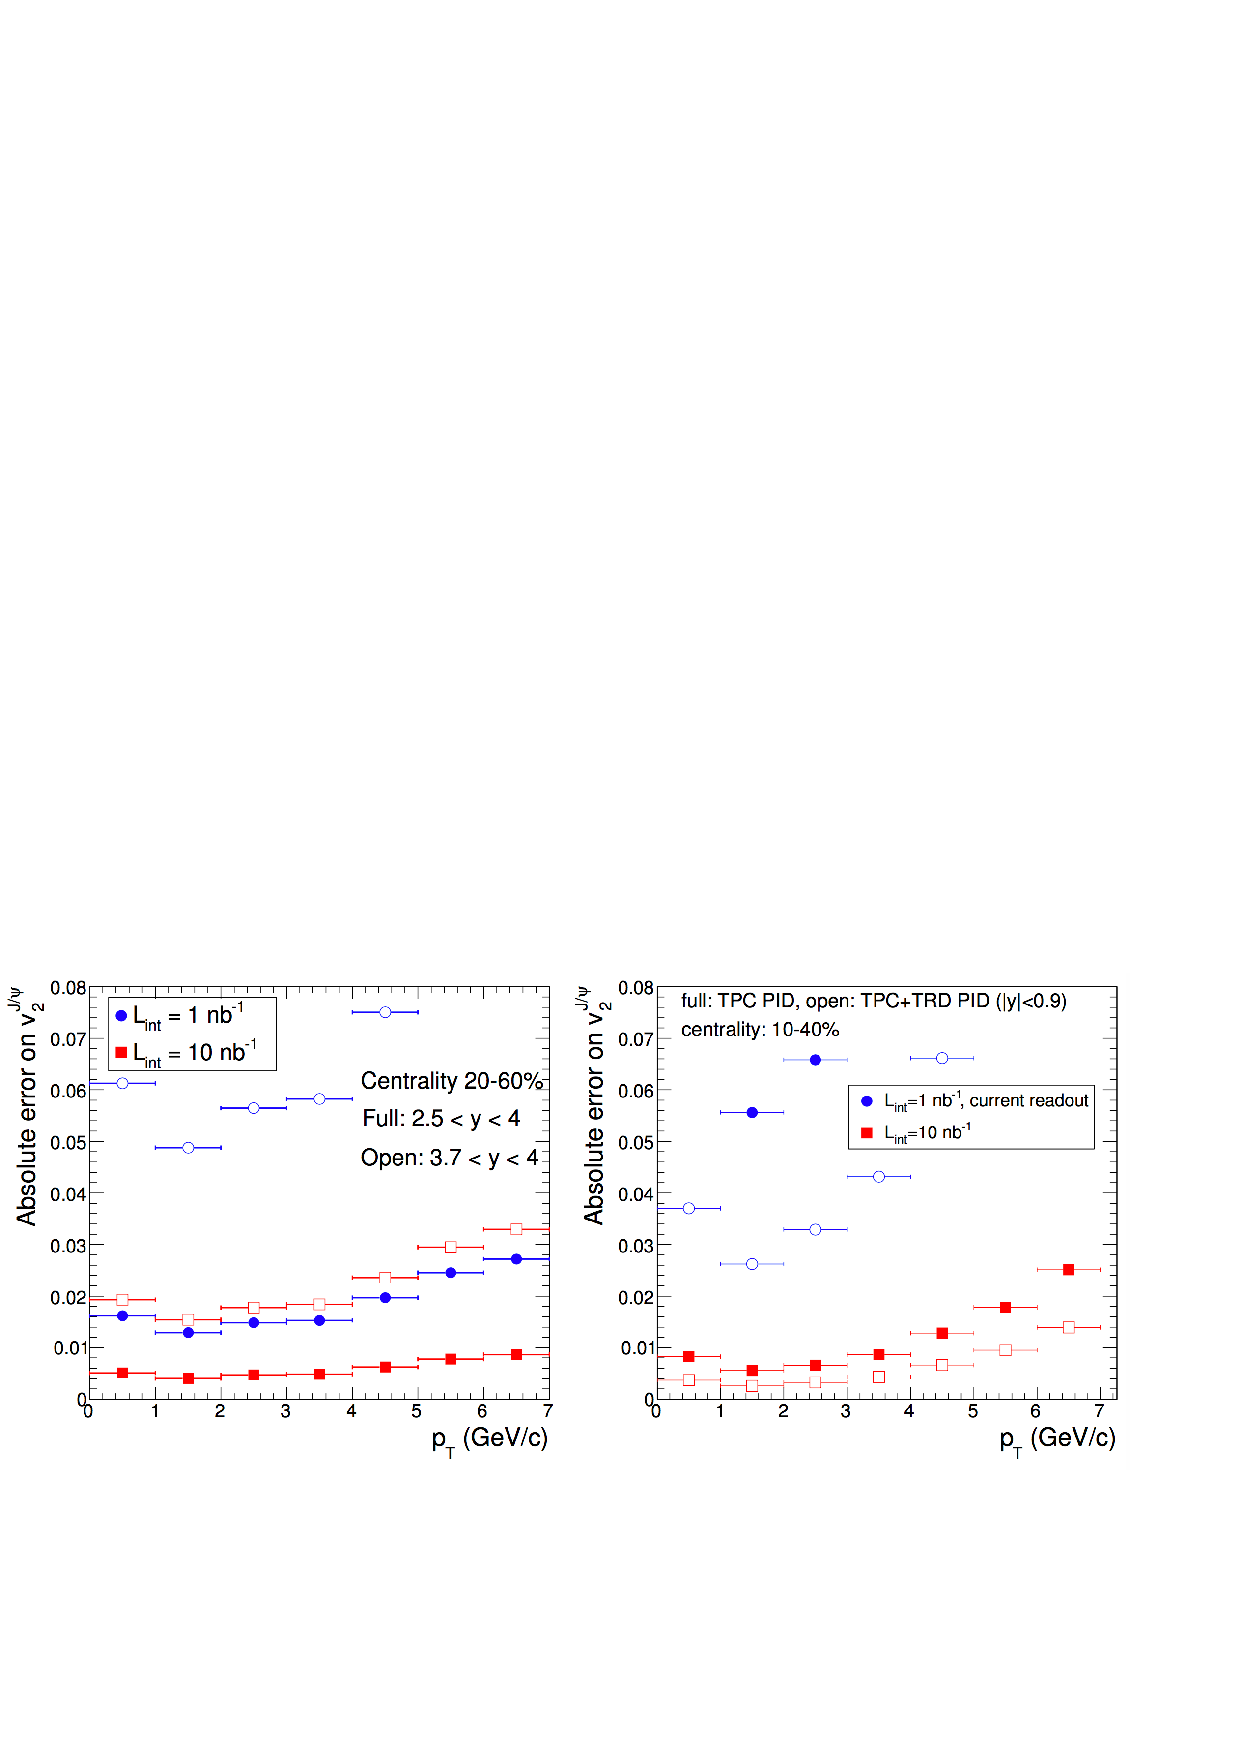
\includegraphics[width=0.66\textwidth]{\main/quarkonia/fig/alice/alice_jpsi_v2_projected.pdf}
 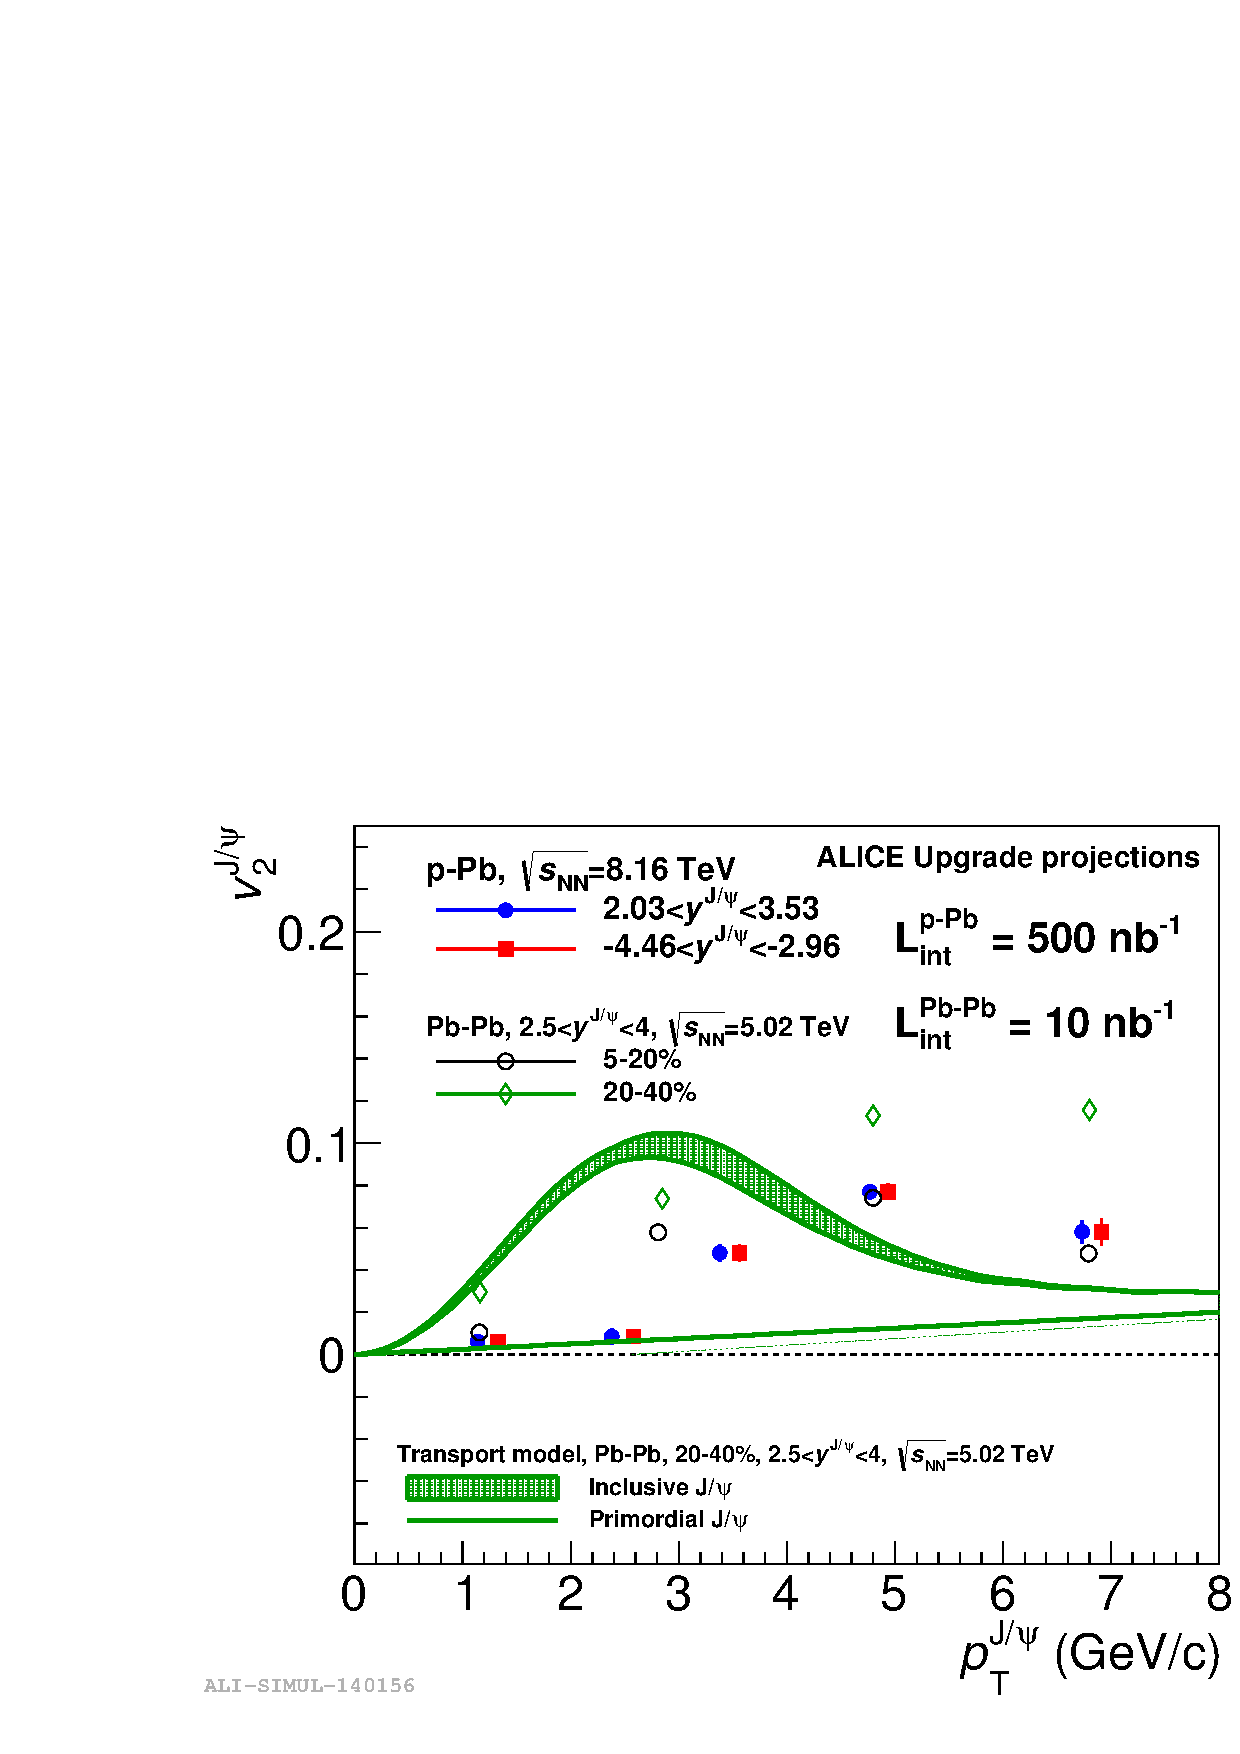
\includegraphics[width=0.32\textwidth]{\main/quarkonia/fig/alice/alice_jpsi_v2_projected2.pdf}
\end{center}

 \caption{prompt J/psi v2 vs \pt, for 30--50\%: $|y|<0.9$, $1.6<|y|<2.4$, $2.5<|y|<4$~\cite{Abelevetal:2014cna,CERN-LHCC-2013-014}}
\end{figure}

\begin{figure}
\begin{center}
 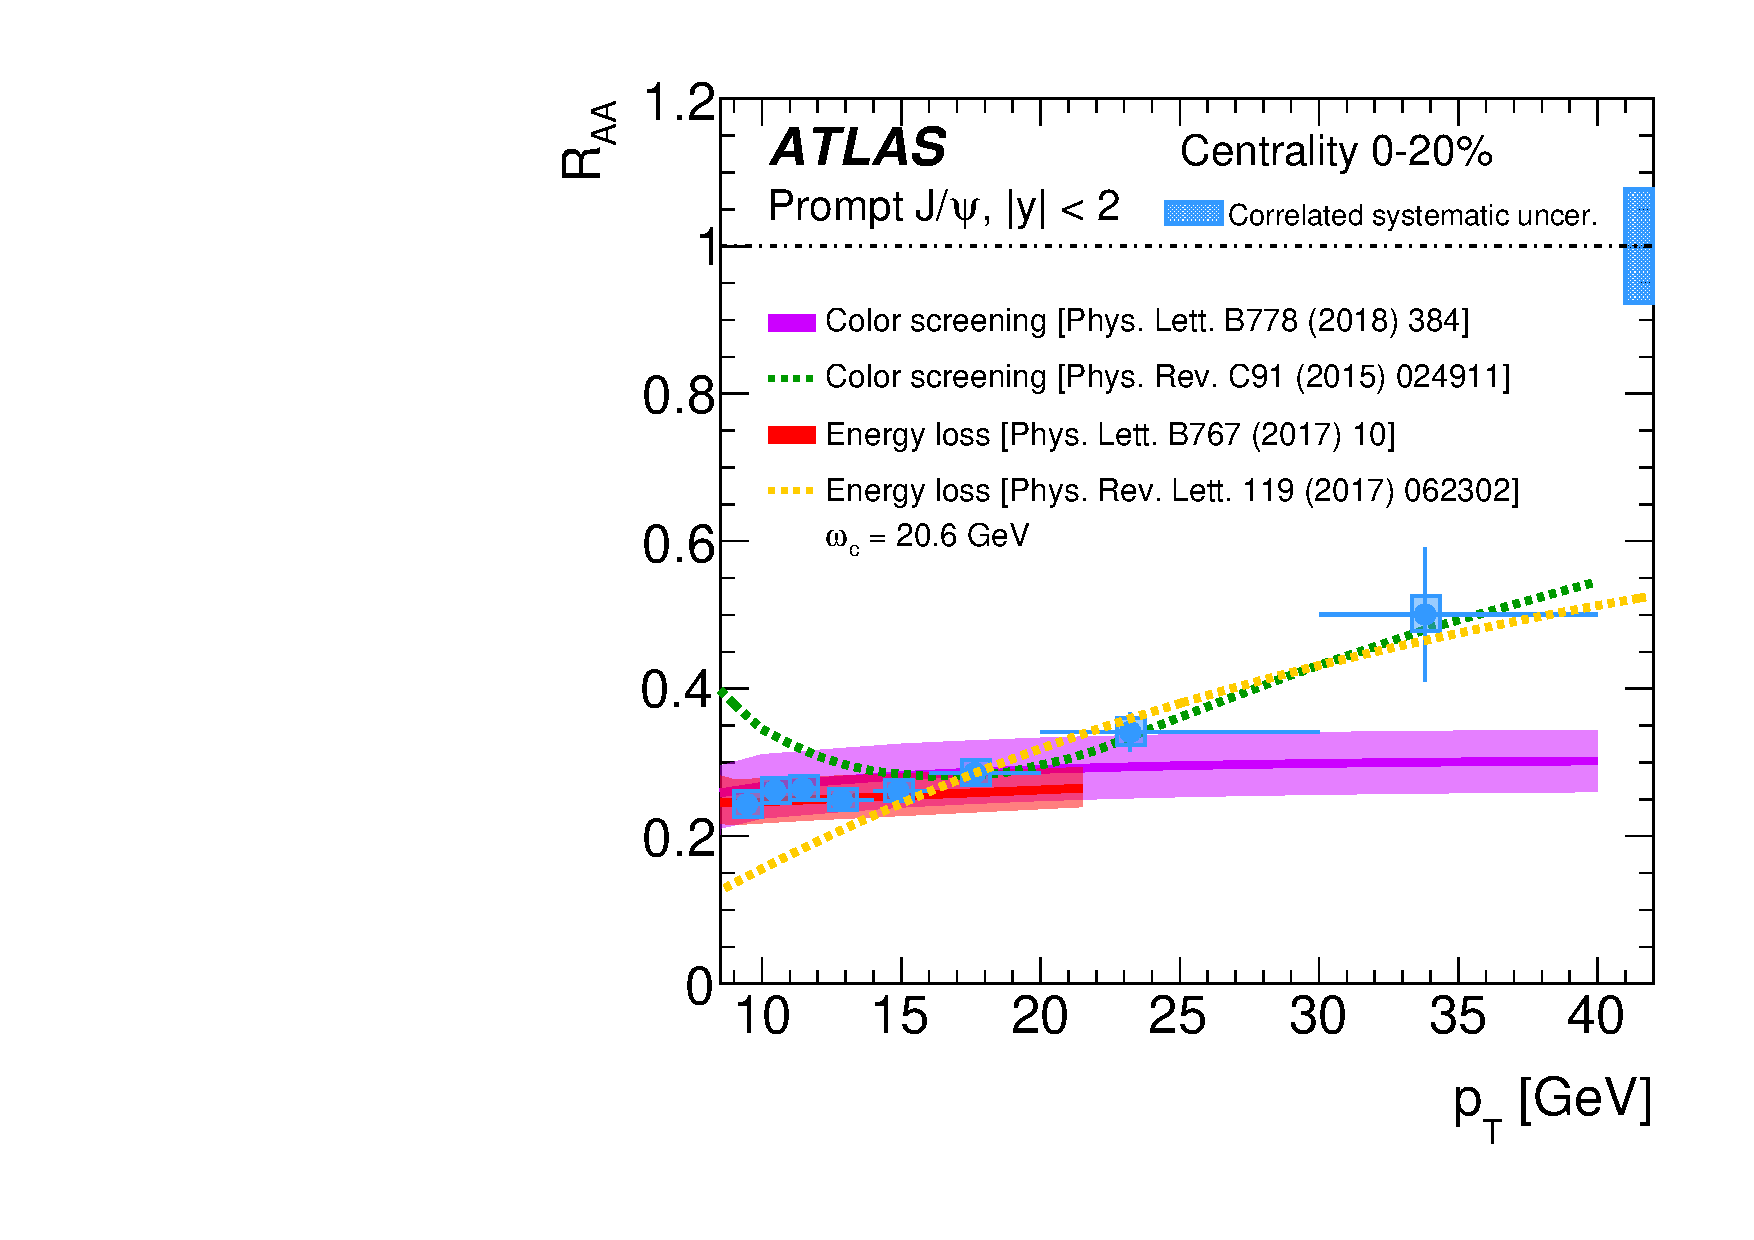
\includegraphics[width=0.5\textwidth]{\main/quarkonia/fig/atlas/atlas_promptjpsi_models}
\end{center}

 \caption{prompt J/psi RAA vs Pt ($|y|<2.4$) at high pT~\cite{Aaboud:2018quy}}
\end{figure}

\begin{figure}
\begin{center}
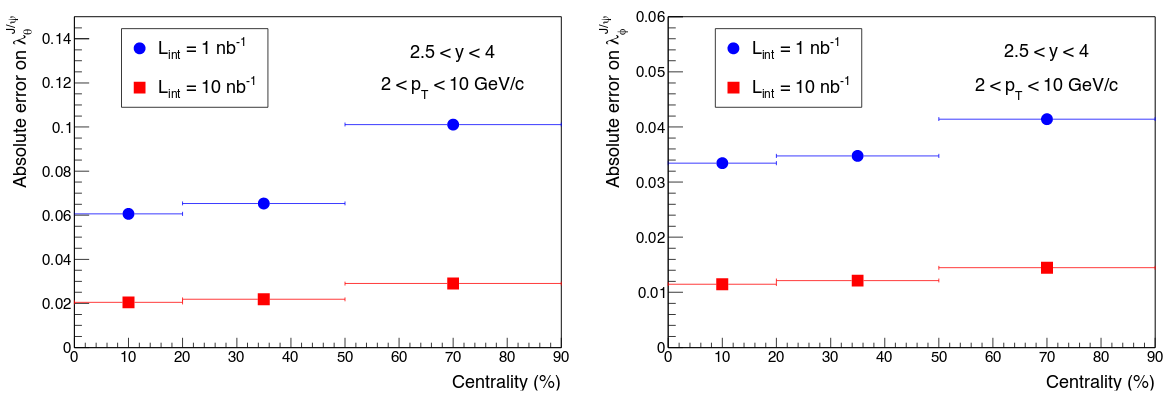
\includegraphics[width=\textwidth]{\main/quarkonia/fig/alice/jpsi_polarisation.png}
\end{center}

 \caption{prompt J/psi polarisation~\cite{Abelev:1475243}}
\end{figure}

\begin{figure}
\begin{center}
 ?
\end{center}

 \caption{prompt psi(2S) RAA (and yields) vs. Npart (pT integrated) }
\end{figure}

\begin{figure}
\begin{center}
% 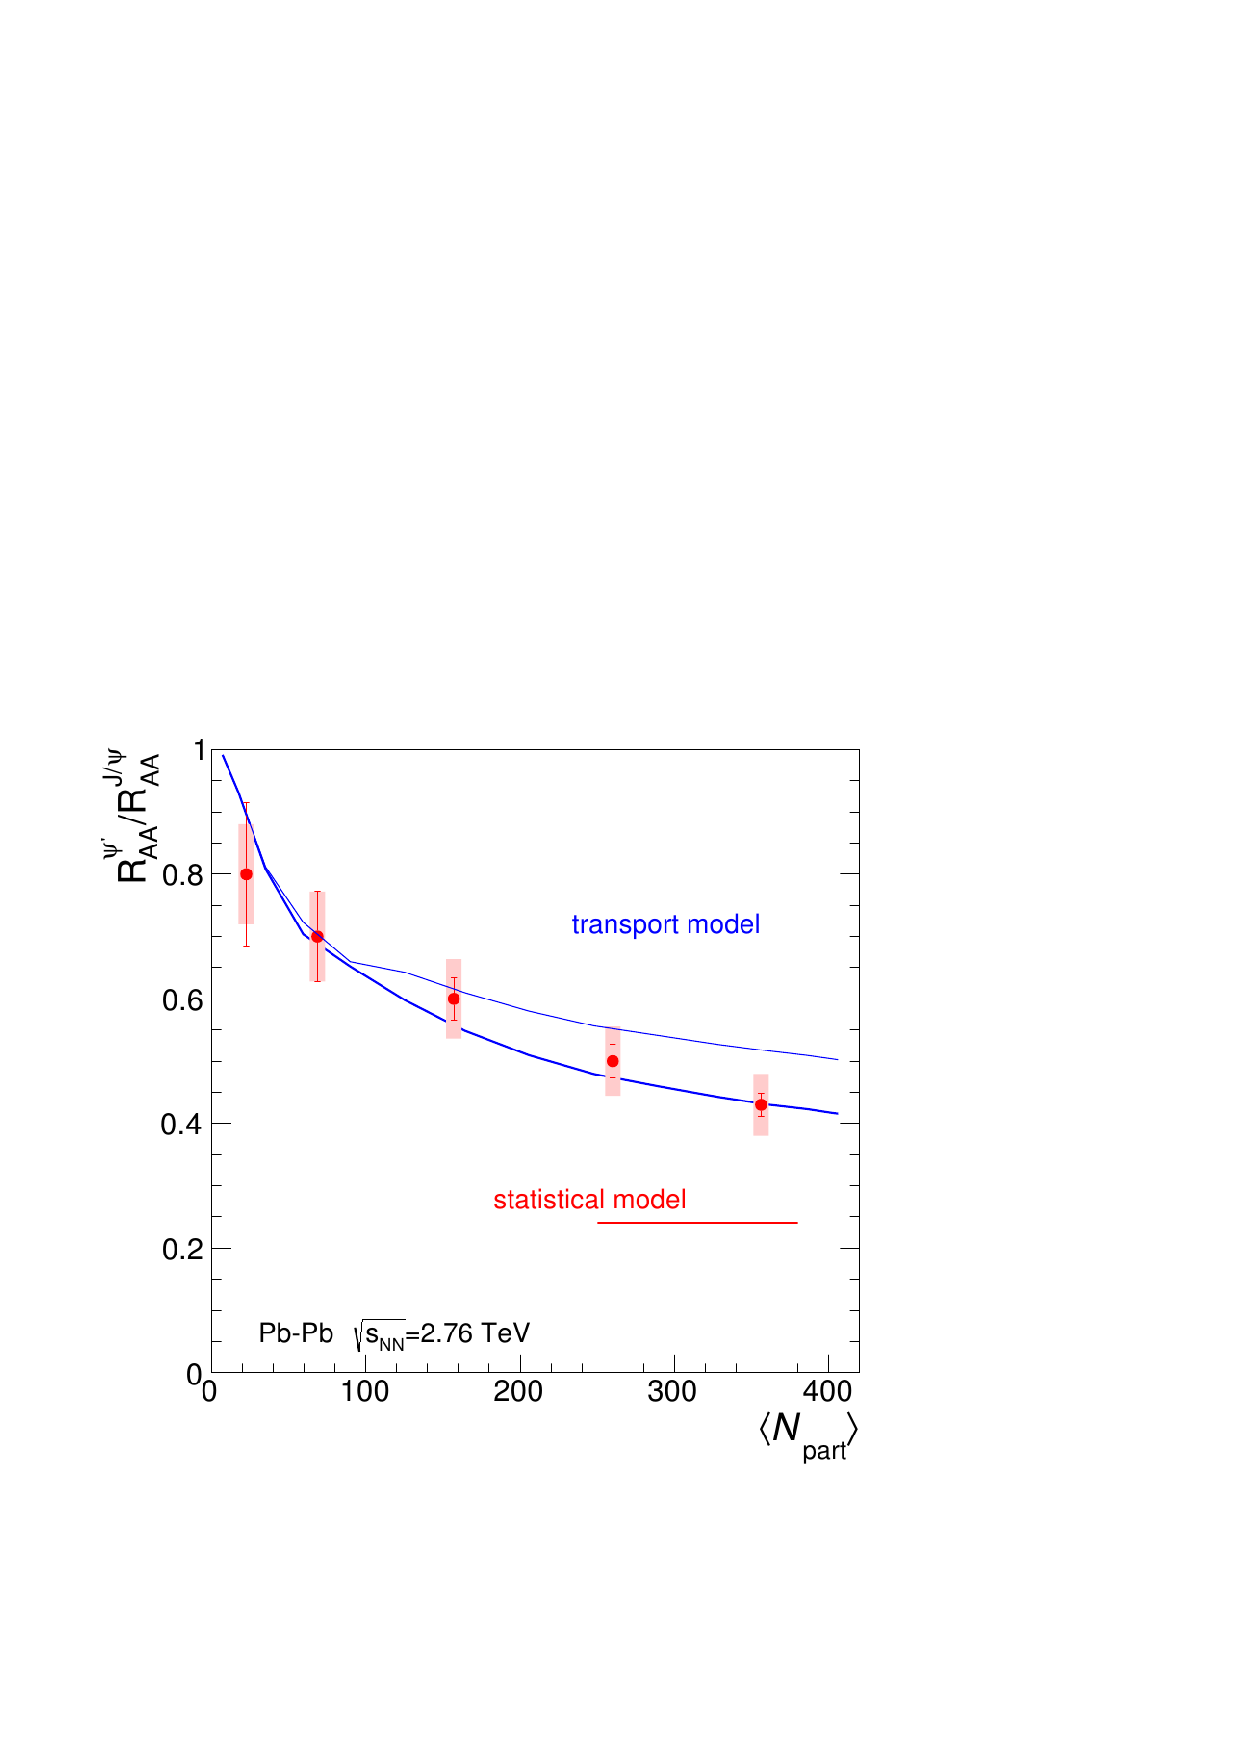
\includegraphics[width=0.32\textwidth]{\main/quarkonia/fig/alice/alice_dr_psi_projected}
% 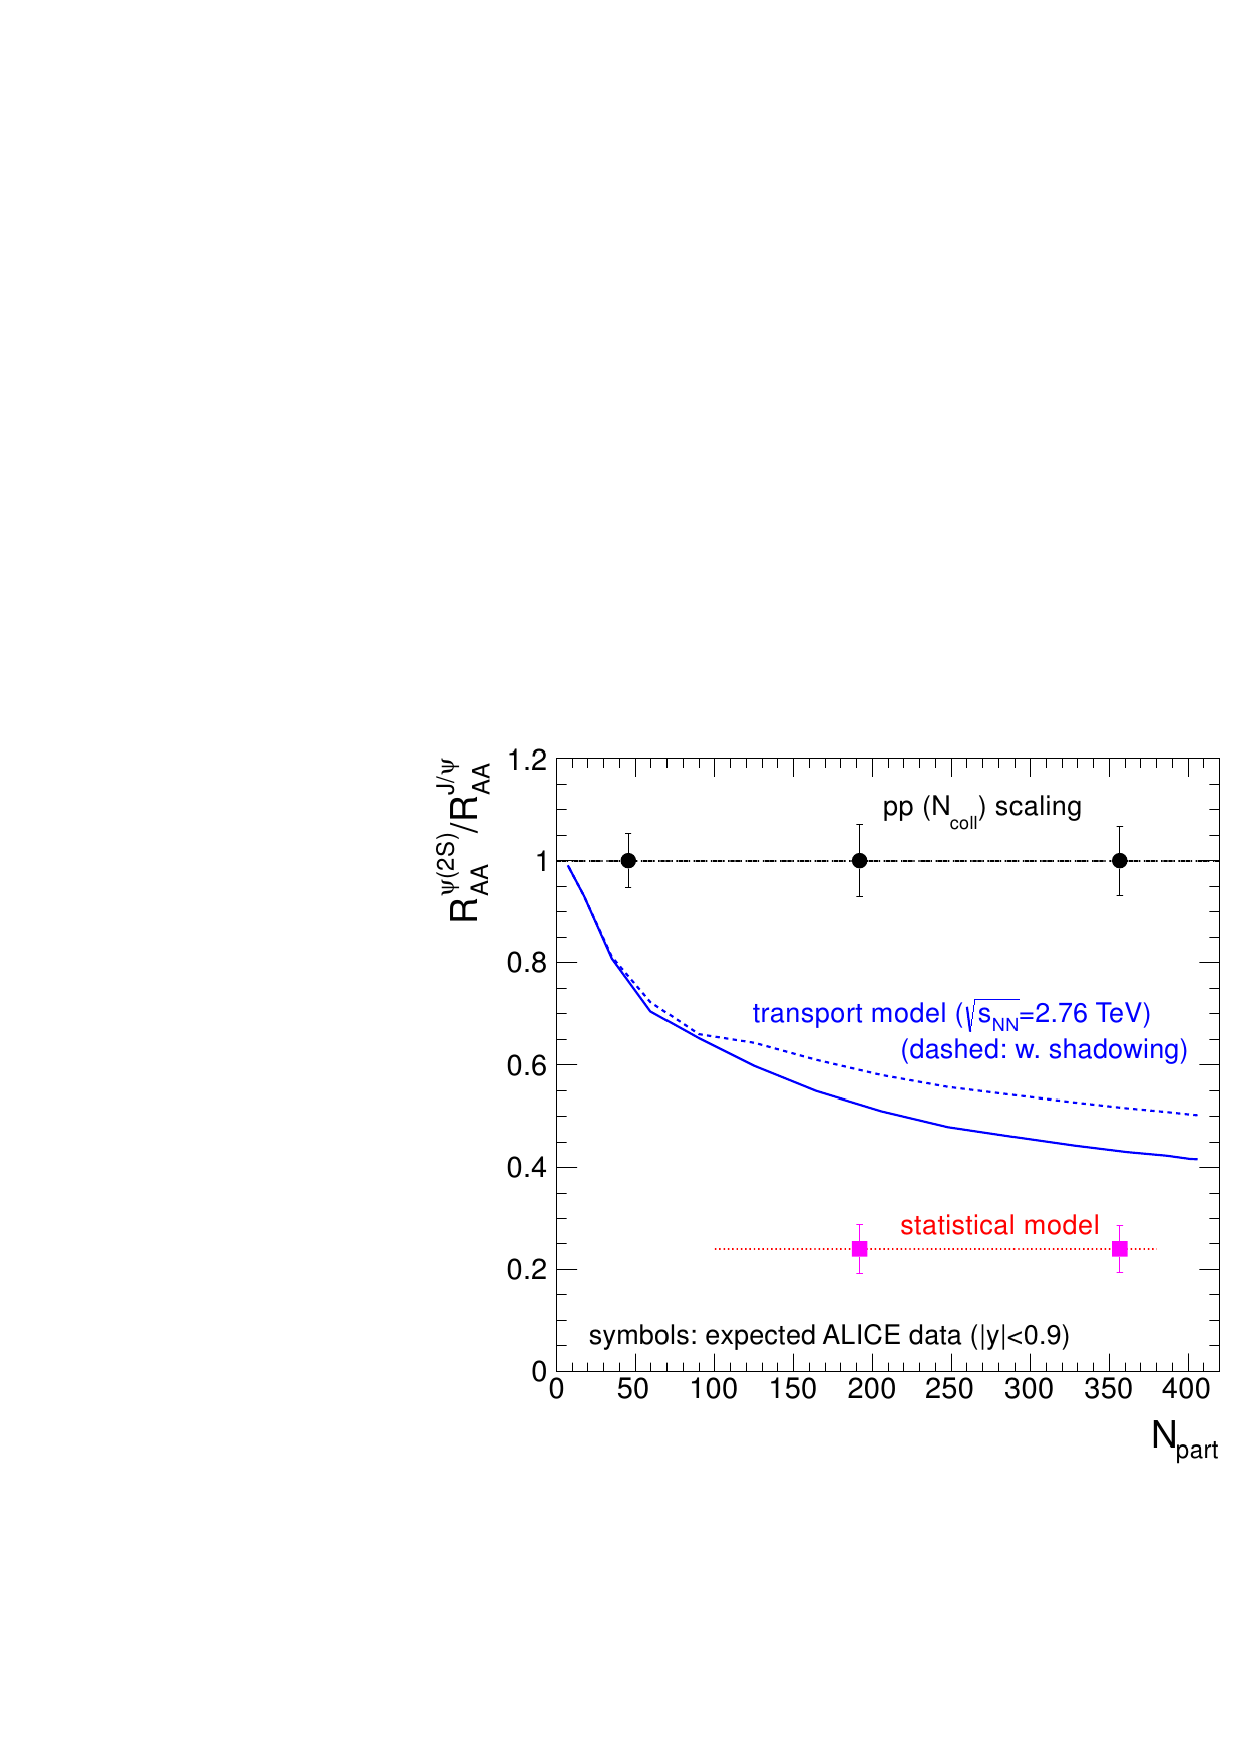
\includegraphics[width=0.32\textwidth]{\main/quarkonia/fig/alice/alice_dr_psi_projected2}
\end{center}

 \caption{prompt psi(2S)/J/psi (or psi2S RAA) vs. Npart: $|y|<0.9 (2.4)$, $2.5<|y|<4$}
\end{figure}

\begin{figure}
\begin{center}
 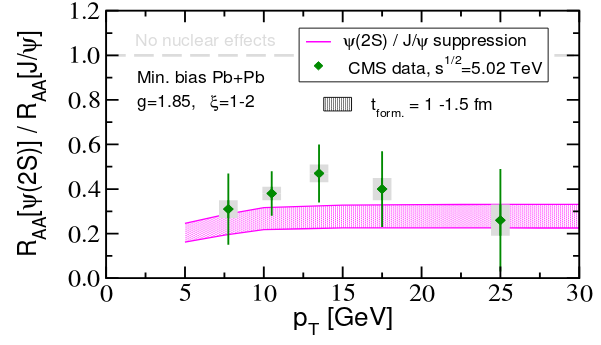
\includegraphics[width=0.32\textwidth]{\main/quarkonia/fig/theory/psi_dr_vitev.png}
\end{center}

 \caption{prompt psi(2S) (and J/psi, or ratio) vs. pT (at low and high pT) }
\end{figure}

\begin{figure}
...

 \caption{prompt psi(2S) v2 vs pT for 30--50\%}
\end{figure}

\begin{figure}
\begin{center}
 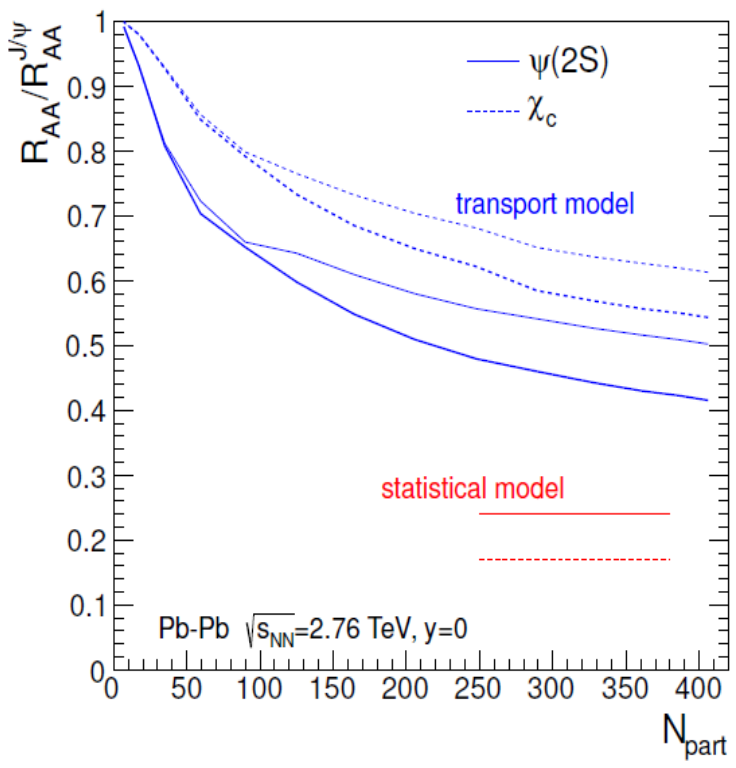
\includegraphics[width=0.32\textwidth]{\main/quarkonia/fig/theory/chic.png}
\end{center}

 \caption{RAA of chic(1P), X(3872) vs pT for $|y|<2.4$}
\end{figure}

\clearpage

\subsection{Bottomonia in PbPb collisions (Main contributor: Emilien Chapon)}

% To cite: Strickland papers, Rapp papers, Nora, Debasish, exp. papers...

% Intro about bottomonia: specificities wrt charmonia, overview of theoretical ingredients.
% Mass, beauty vs charm, 3 states, Tdiss, no B feed-down, feed-down, ...
% split in th vs exp differences
The study of bottomonia with \PbPb data from the Runs 3 and 4 of the LHC can bring further information on the various physics aspects described above, and more.
Although their production is a priori subject to the same effects as charmonia, in practice the two quarkonium families feature some fundamental differences.
Binding energies differ, which is reflected in the different dissociation temperatures: about twice the critical temperature $T_C$ for \PGUP{1S}, much high than the about
$1.2 T_C$ for \PJgy or \PGUP{2S}, for instance. The feed-down pattern is also more complex: while the contribution of B meson decays is specific to charmonia, more states can
contribute to the different $S$-wave bottomonia, owing to decays of \PGUP{2S} and \PGUP{3S}, as well as the many states of the \PGcb family. In practice, up to $30-40$\% of the measured 
\PGUP{1S} and \PGUP{2S} yields actually result from the feed-down from other states. At the same time, this important feature of bottomonium production means that
a large portion of measured \PGUP{1S} suppression can be due to the stronger suppression of the feed-down states.
In addition, the feed-down fractions, for the contribution of the 
different states to the measured bottomonium states, are constrained experimentally as a function of $\pt$ but with limited precision, which is one source of uncertainty in the models.
The impact of regeneration from uncorrelated $\text{b}\bar{\text{b}}$ is also expected to be much smaller than for charmonia, because of the much smaller number of $\text{b}\bar{\text{b}}$
pairs per \PbPb event compared to $\text{c}\bar{\text{c}}$. The importance of regeneration for bottomonia is however still very model dependent, and no unambiguous experimental signal
for it has been found yet. Possible ways of constraining this contribution will be discussed in this section.

Experimentally, the higher mass of bottomonia compared to charmonia implies higher $\pt$ decay leptons, allowing the ATLAS and CMS experiments to measure the production down to 0 $\pt$,
as is possible for ALICE for both charmonia and bottomonia. The proximity in mass between the different mass states, especially between the \PGUP{2S} and \PGUP{3S} states, also 
means that good muon (or electron) momentum resolution is essential to their measurement, especially for excited states. 
% , while the addition of the MFT will also beneficial in improving the muon momentum resolution of the ALICE detector.

% Summary of Run1+Run2 results 
It is useful to remind quickly the status in 2018, based on results from Run1 and early Run2 LHC data as well as RHIC data. \PGU production is found to be suppressed in \PbPb compared to \pp
collisions, in all rapidity, $\pt$ and centrality ranges measured. Suppression is stronger in central events, as expected from the hotter and longer-lived medium in such events.
Another striking feature is that excited states are more suppressed than the ground state, the \PGUP{3S} being still unmeasured in AA collisions ($\raa(\PGUP{3S})<0.094$ at 95\% confidence
level, for $\sqrtsnn = \unit[5.02]{TeV}$~\cite{Sirunyan:2018nsz}). In addition, the large suppression found for \PGUP{1S} in central collisions does not seem compatible with unmodified direct \PGUP{1S} production,
though uncertainties on non-QGP effects (initial state modifications and final state effects) do not allow for an undebatable statement regarding \PGUP{1S} melting in the medium.
No significant dependence of the suppression of \PGU states is found on collision energy or rapidity.

Experimentally, the main provision of Runs 3 and 4 data, compared to Runs 1 and 2, will be the much higher quantity of data, expected to be \unit[10]{nb}$^{-1}$, an increase of a factor about
100 for the ALICE experiment %FIXME check
and about 5 for the ATLAS and CMS experiments. The much higher precision will be most beneficial in regions of the phase space where the cross section is smaller: for instance at
forward rapidity and in peripheral collisions. At the same time, there is access to higher $\pt$ bottomonia, up to about 50\,GeV with ATLAS and CMS, where one could look for hints of an
increasing \raa, as found for prompt \PJgy in Run~2 data~\cite{Sirunyan:2017isk,Aaboud:2018quy}. In addition, more data will be even more appreciable for \PGUP{2S} and \PGUP{3S}: 
the modification of the former in \PbPb collisions is known with limited precision today, and only upper limits on the production of the latter are available. More data will also have
an impact on the main systematic uncertainties impacting results today. Efficiency uncertainties will be reduced, thanks to the larger calibration datasets recorded (minimum bias data
and \PJgy data for tag-and-probe corrections). At the same time, uncertainties on the modelling of signal and background mass shapes will also be reduced, some unrealistic 
parametrisations being rejected by the more precise data.

% comments on Phase-I and Phase-II upgrades
The addition of the Muon Forward Tracker (MFT) during LS2 will also impact \PGU measurements from ALICE. The main improvement will be a reduction in the background, yielding to better signal over background
ratios. This will further improve the precision for \PGUP{1S} measurements, as well as enable differential $\PGUP{2S}+\PGUP{3S}$ measurements.
In addition, the ATLAS and CMS detectors will also undergo major upgrades between Runs 3 and 4, with an inner tracker
extending to $|\eta|\lesssim 4.0$ (3.8) for ATLAS (CMS), and with extended muon coverage to $|\eta|\lesssim 2.7$ (3.0). While the detector improvements will have a smaller impact than the
increase in statistics, this increase in pseudorapidity coverage is appreciable in also giving an overlap with the range of ALICE and LHCb.

% Discuss regeneration

\begin{figure}
\begin{center}
 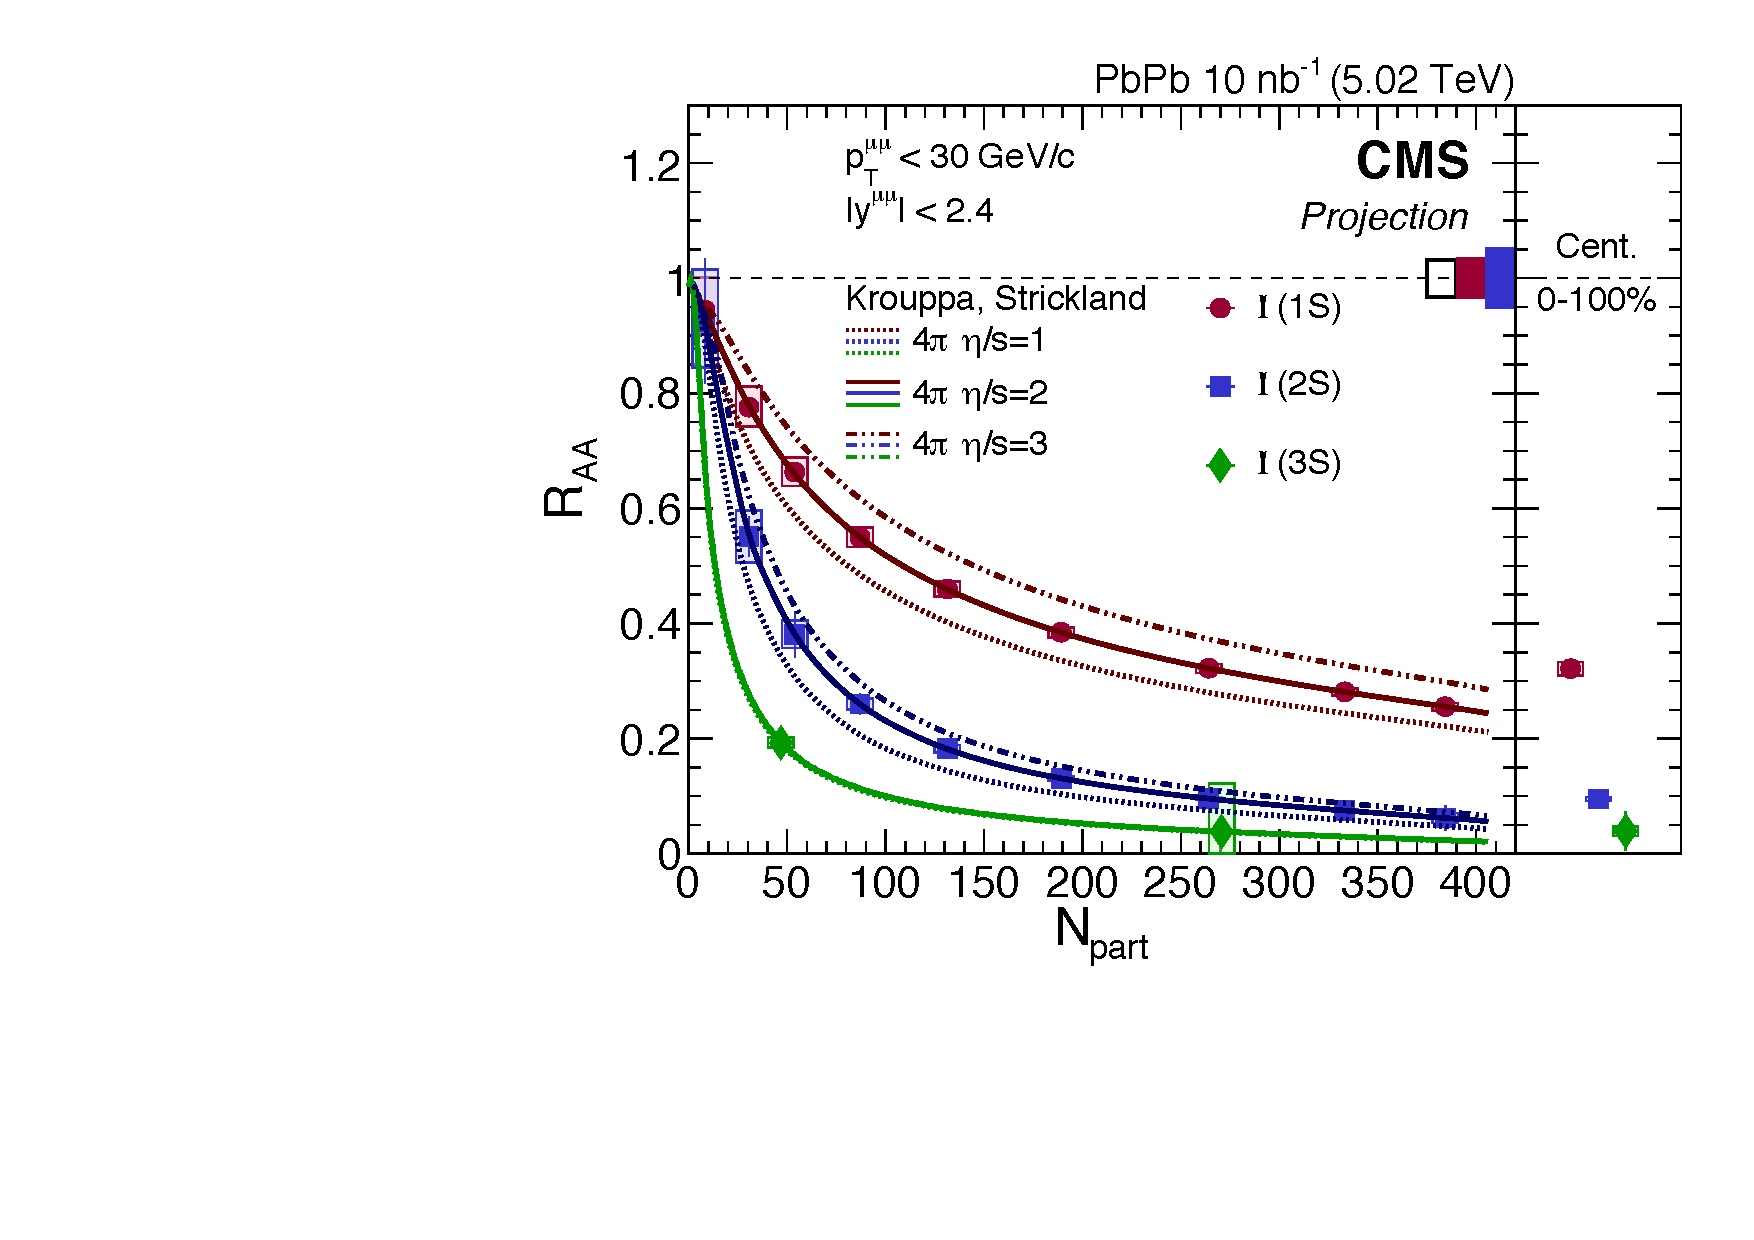
\includegraphics[width=0.32\textwidth]{\main/quarkonia/fig/cms/CMS-PAS-FTR-17-002_Figure_008-b.pdf}
 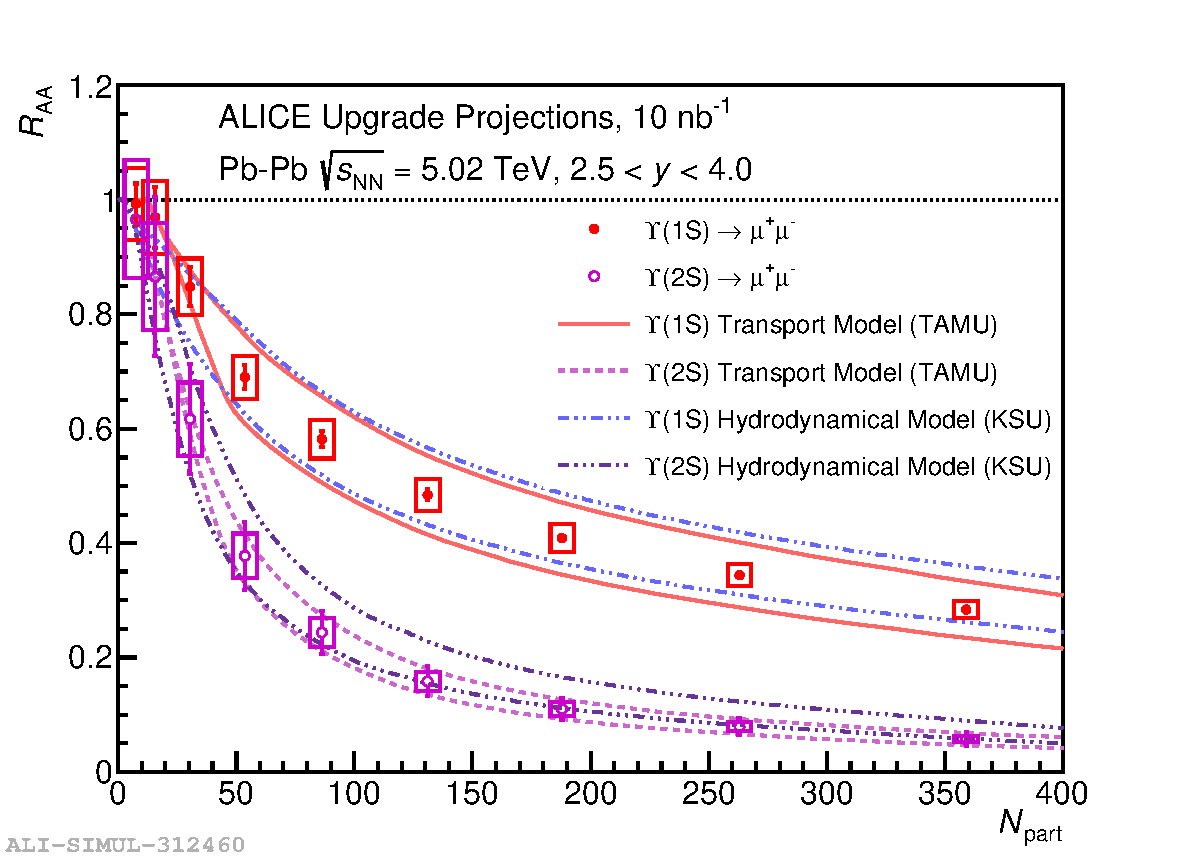
\includegraphics[width=0.32\textwidth]{\main/quarkonia/fig/alice/craa_cent}
 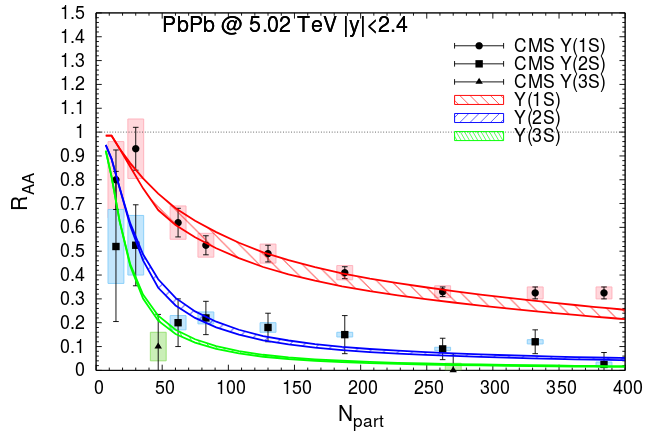
\includegraphics[width=0.32\textwidth]{\main/quarkonia/fig/theory/rapp_raa_npart_CMS.png}
\end{center}

 \caption{Centrality dependence of \PGUP{1}, \PGUP{2} and \PGUP{3} \raa, as projected by the CMS\cite{CMS-PAS-FTR-17-002,Krouppa:2016jcl} (left) and ALICE (centre) experiments, and from a transport model\cite{Du:2017qkv}}
 \label{fig:upsi_raa_npart}
\end{figure}

% \begin{figure}
%  \begin{center}
%   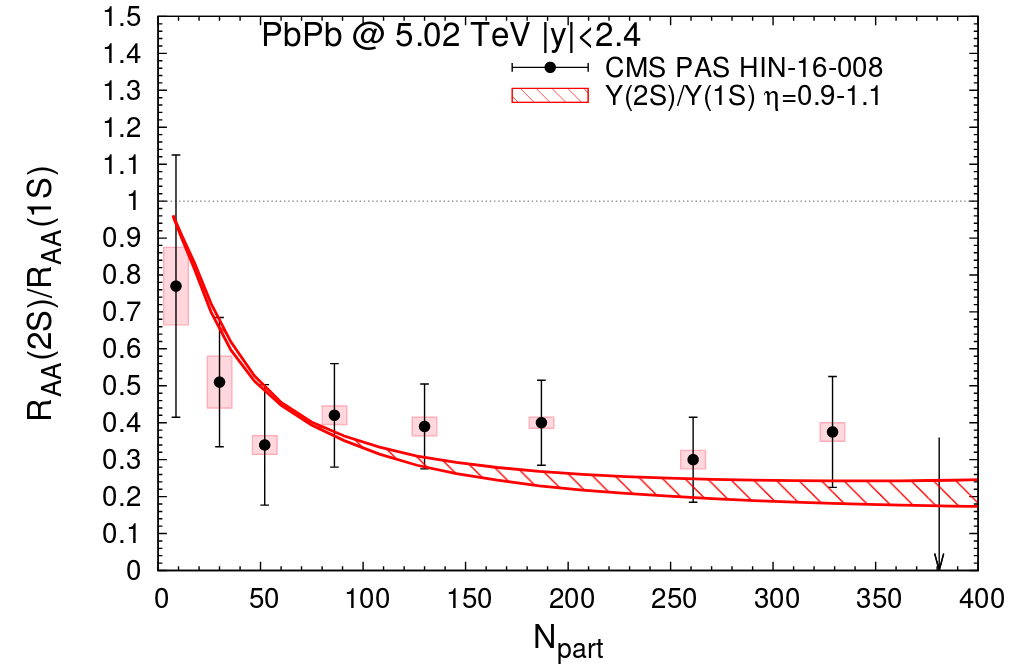
\includegraphics[width=0.32\textwidth]{\main/quarkonia/fig/theory/rapp_dr_npart.png}
%  \end{center}
% 
%  \caption{Y(2S,3S)/Y(1S) vs Npart~\cite{Du:2017qkv}}
% \end{figure}

% discuss centrality dependence: importance of different ingredients... potential, initial T, hydro vs transport, etc

The main striking features of \PGU suppression can be observed in Fig.~\ref{fig:upsi_raa_npart} and in current data: first a strong dependence of the suppression with the collision
centrality, with a stronger suppression in the most central collisions, and also a higher suppression of the excited states compared to the ground state. Good qualitative agreement
is already found between models and data regarding this suppression, within current uncertainties. Figure~\ref{fig:upsi_raa_npart} shows the the projected uncertainty on the \raa of \PGUP{1} will be much smaller than the current model uncertainties.

Differences exist however in the treatment of the suppression of the bottomonia in the medium.
For instance, the heavy quark potential, qualitatively a Debye screened potential above the deconfinement temperature, as proposed originally~\cite{Matsui:1986dk}, is one important
ingredient. Some models assume a real potential, using usually the free energy or the internal energy (as in Ref.~\cite{Du:2017qkv}). More recently, developments from lattice lQCD
have allowed to also study the imaginary part of the potential, which physics implications are under study but may be related to Landau damping and singlet-octet transitions. Through the 
use of such lQCD-vetted potential, it has been shown~\cite{Krouppa:2017jlg} that predictions are quite sensitive to this choice, as compared to a perturbative potential. 

Models also differ in the treatment of the evolution of the quarkonia with the medium. Frameworks include a transport model with a kinetic-rate equation~\cite{Du:2017qkv},
anisotropic hydrodynamics~\cite{Krouppa:2017jlg}, comovers~\cite{Ferreiro:2018wbd}, effective field theory in the framework of open quantum systems with 
a Lindblad equation~\cite{Brambilla:2017zei}. Precise predictions require many other ingredients. Some can be constrained using measurements in \pp collisions, such as
the feed-down fractions from other states, or in \pPb collisions for cold nuclear matter and initial state effects (including nPDF). In other cases, bottomonia may bring information
complementary to other probes, using the sensitivity of the suppression to the medium shear viscosity or to its initial temperature.

\begin{figure}
\begin{center}
 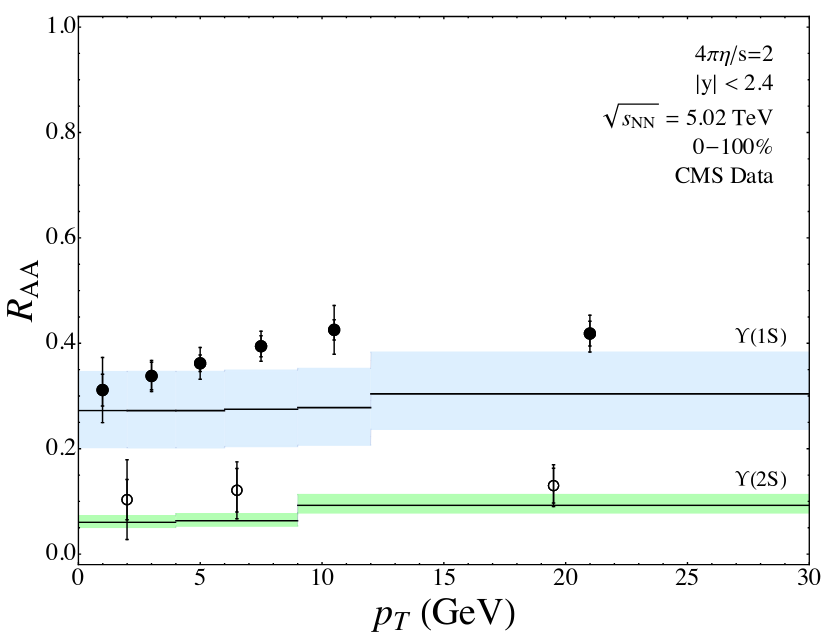
\includegraphics[width=0.32\textwidth]{\main/quarkonia/fig/theory/strickland_pt.png}
 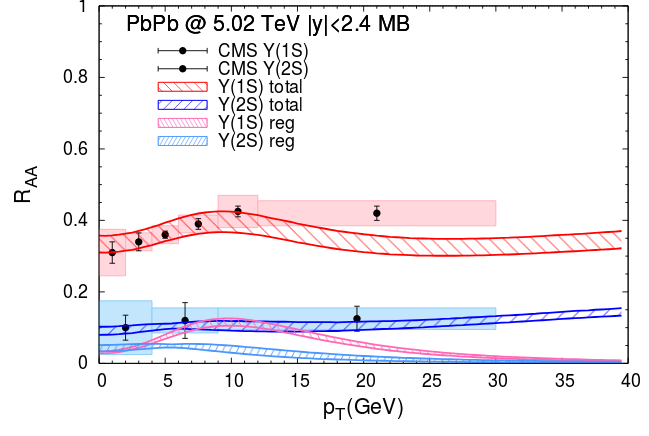
\includegraphics[width=0.32\textwidth]{\main/quarkonia/fig/theory/rapp_raa_pt_CMS.png}
 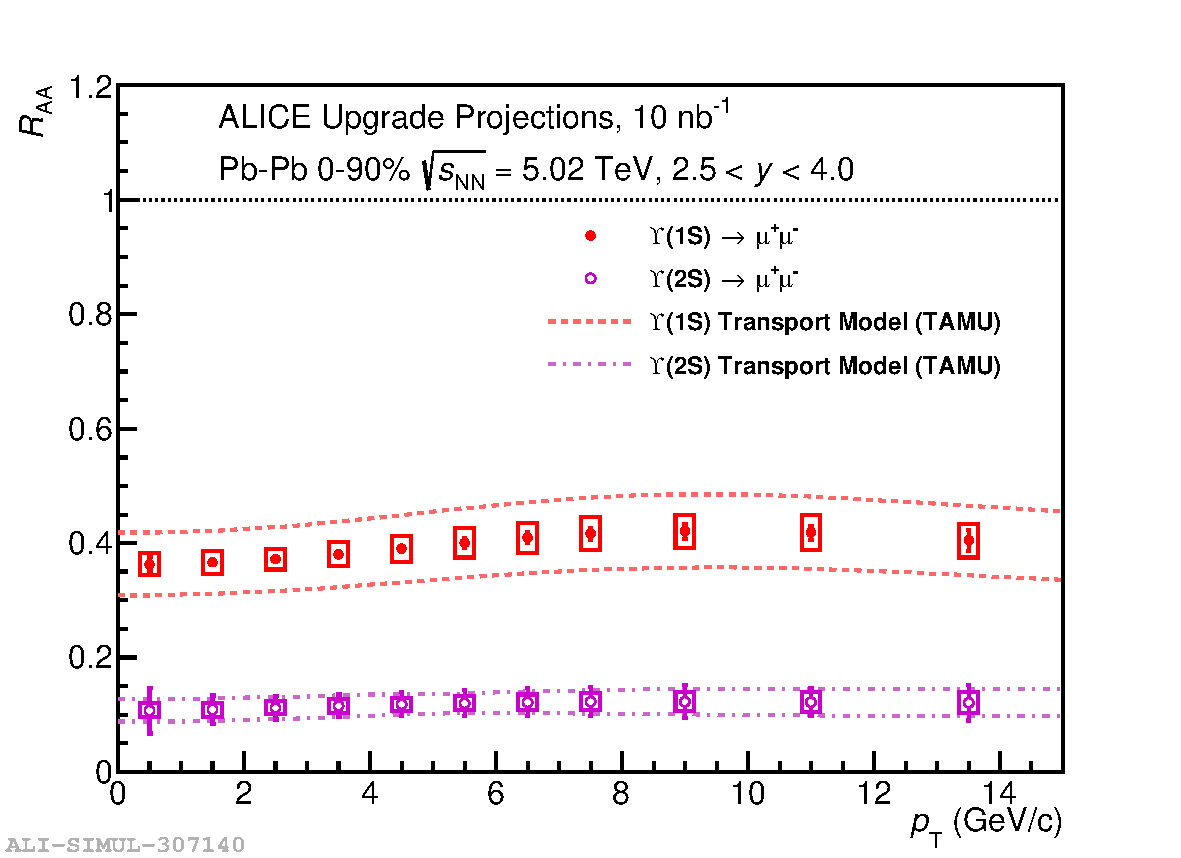
\includegraphics[width=0.32\textwidth]{\main/quarkonia/fig/alice/craa_pt}
 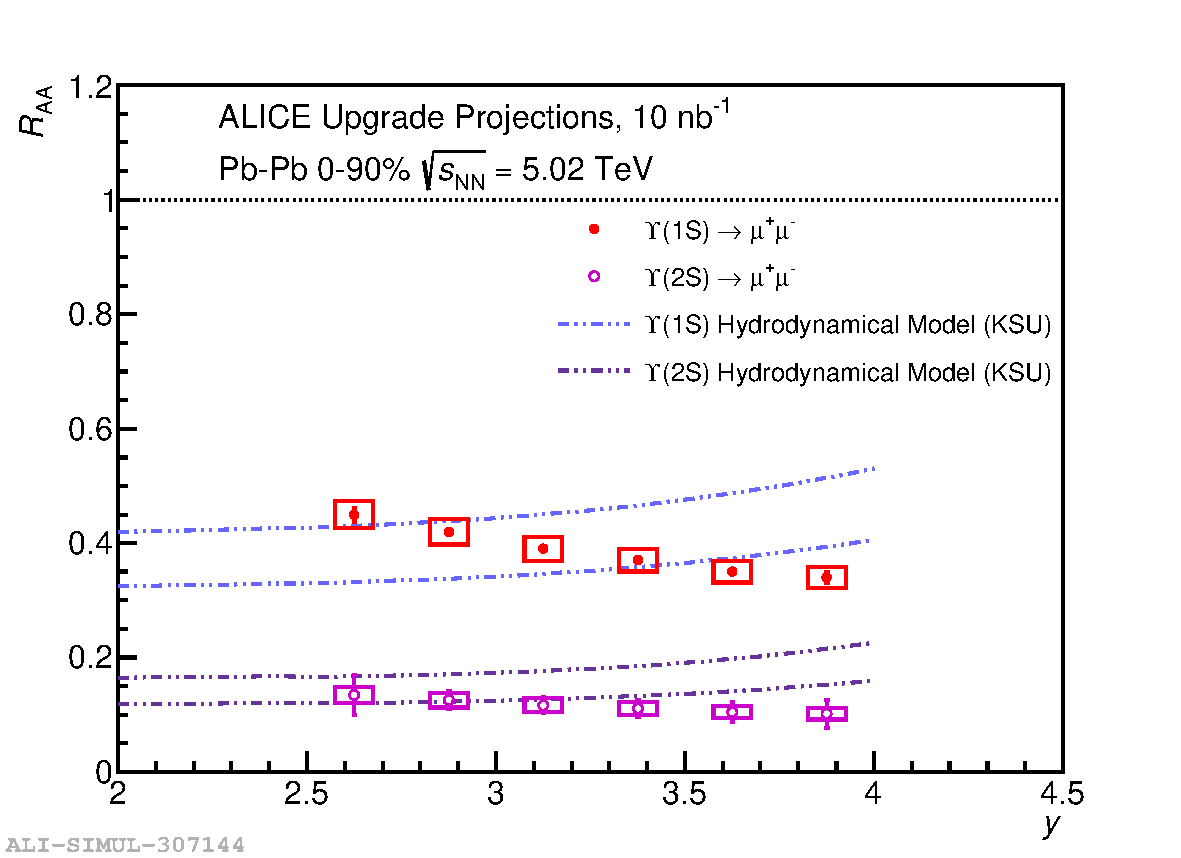
\includegraphics[width=0.32\textwidth]{\main/quarkonia/fig/alice/craa_y}
 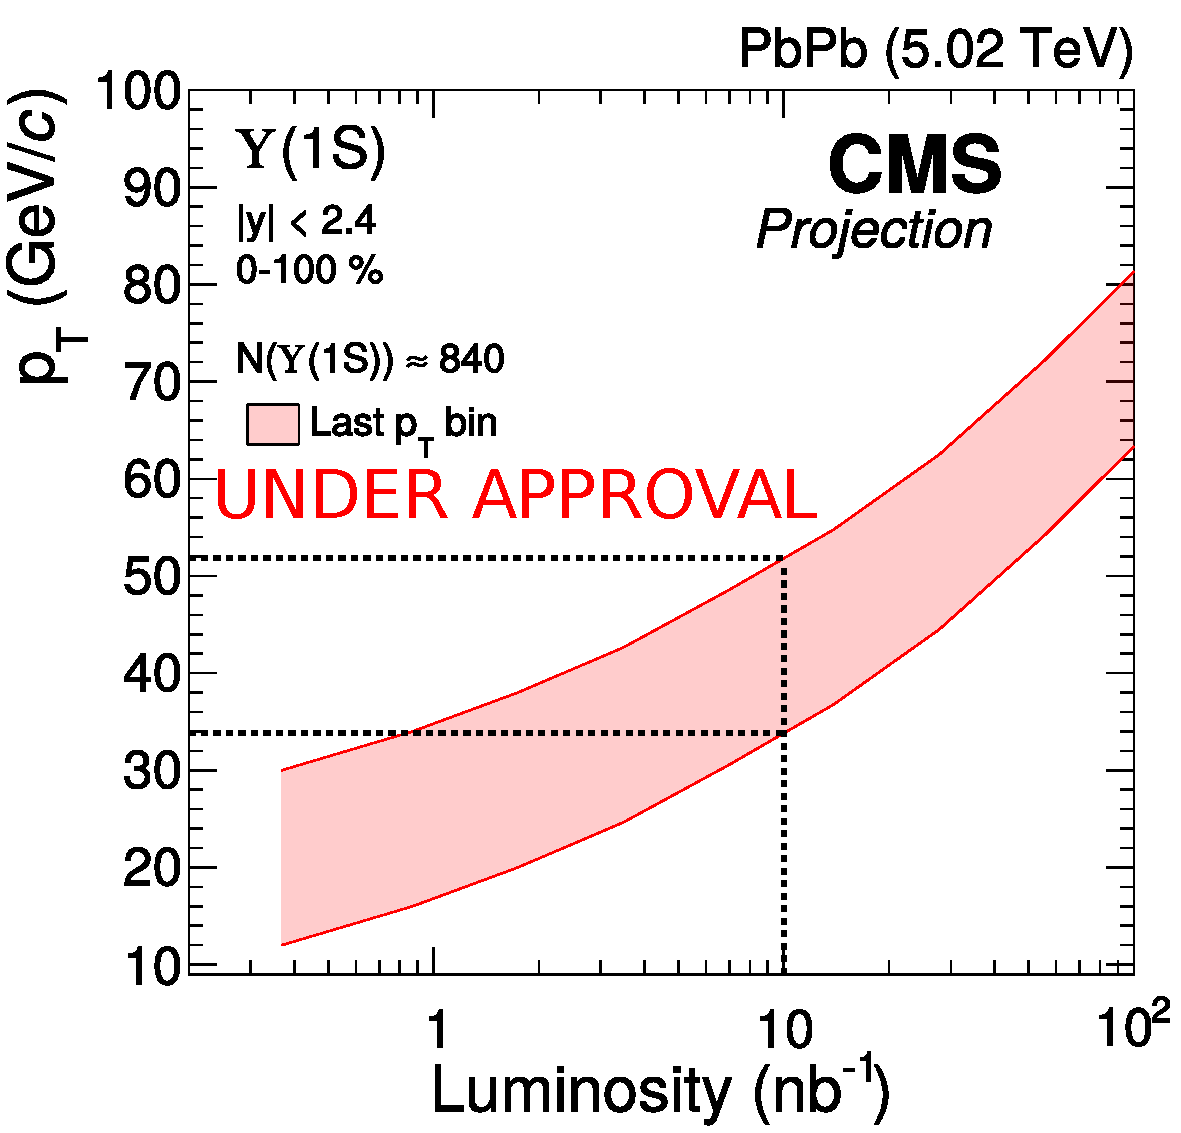
\includegraphics[width=0.32\textwidth]{\main/quarkonia/fig/cms/Upsilon1S_pTvsLumi}
\end{center}

 \caption{\raa vs $\pt$, \raa vs y for 0--10\%, 0--100\%~\cite{Krouppa:2017jlg,Du:2017qkv} ALICE projections are NOT APPROVED yet, as well as CMS high pt
 }
 \label{fig:upsi_raa_pt_y}
\end{figure}

% Discuss pt / y dependence with boost... what we learn from it (also regeneration)
A precise measurement of the $\pt$ dependence of the \PGUP{1S} \raa will be possible using LHC data from Runs 3 and 4. At low and medium $\pt$, up to about 15\UGeV, the measurement is
sensitive to the possible regeneration component in \PGU meson production. Some projections for the expected precision of \PGU measurements from the ALICE and CMS detectors
using 10\,nb$^{-1}$ of data after the Runs 3-4 are shown in Fig.~\ref{fig:upsi_raa_pt_y} as a function of $\pt$ and y, and compared to the expectations from two 
models~\cite{Krouppa:2017jlg,Du:2017qkv}. In the first model~\cite{Krouppa:2017jlg}, all the measured \PGU are from the primordial production and there is no regeneration, leading
to a rather flat \raa at low and medium $\pt$. Only at higher $\pt$ is a small rise predicted, which will be discussed below. In the second model~\cite{Du:2017qkv} however, a regeneration
component is considered, and several assumptions are explored, especially on the degree of thermalisation of the bottom quarks. Indeed, because of the about three times higher mass of
the bottom quark than that of the charm quark, it cannot be assumed that regenerated bottomonia would have a thermal blast-wave expression, as is a good approximation for charmonia.
In Fig.~\ref{fig:upsi_raa_pt_y}, the latter model uses an instantaneous coalescence model instead, providing more realistic nonequilibrium $\pt$ spectra for the input b quarks. 
This leads to a maximum in the \raa as a function of $\pt$, at around 10\,GeV for \PGUP{1S}. The current data is not precise enough to confirm or disfavour this feature, but Run~3+4 
data will allow to look for it.

Almost no rapidity dependence is expected at LHC for the nuclear modification factor of \PGU mesons within the acceptance of ATLAS and CMS ($|\eta|\lesssim 2.5-3$), which can be better
tested using Run~3+4 data. A modest increase is predicted in the acceptance of ALICE, as can be seen in Fig.~\ref{fig:upsi_raa_pt_y}, because of a cooler QGP. Again, this cannot be tested
within the current experimental uncertainties, but can be looked for in future data.

% Discuss high pt
Though not as sensitive as \PJgy to energy loss processes, because of their higher mass implying a lower boost at a given $\pt$, much can be learnt as well from the measurement of
\PGUP{1} at high $\pt$. As can be seen in Fig.~\ref{fig:upsi_raa_pt_y}, it is expected that a measurement up to a $\pt$ of about 50\UGeV can be performed with the ATLAS and CMS detectors with
\unit[10]{nb}$^{-1}$ of data, where a small increase of the \raa is predicted by current models, as can be seen in in Fig.~\ref{fig:upsi_raa_pt_y}.

\begin{figure}
\begin{center}
 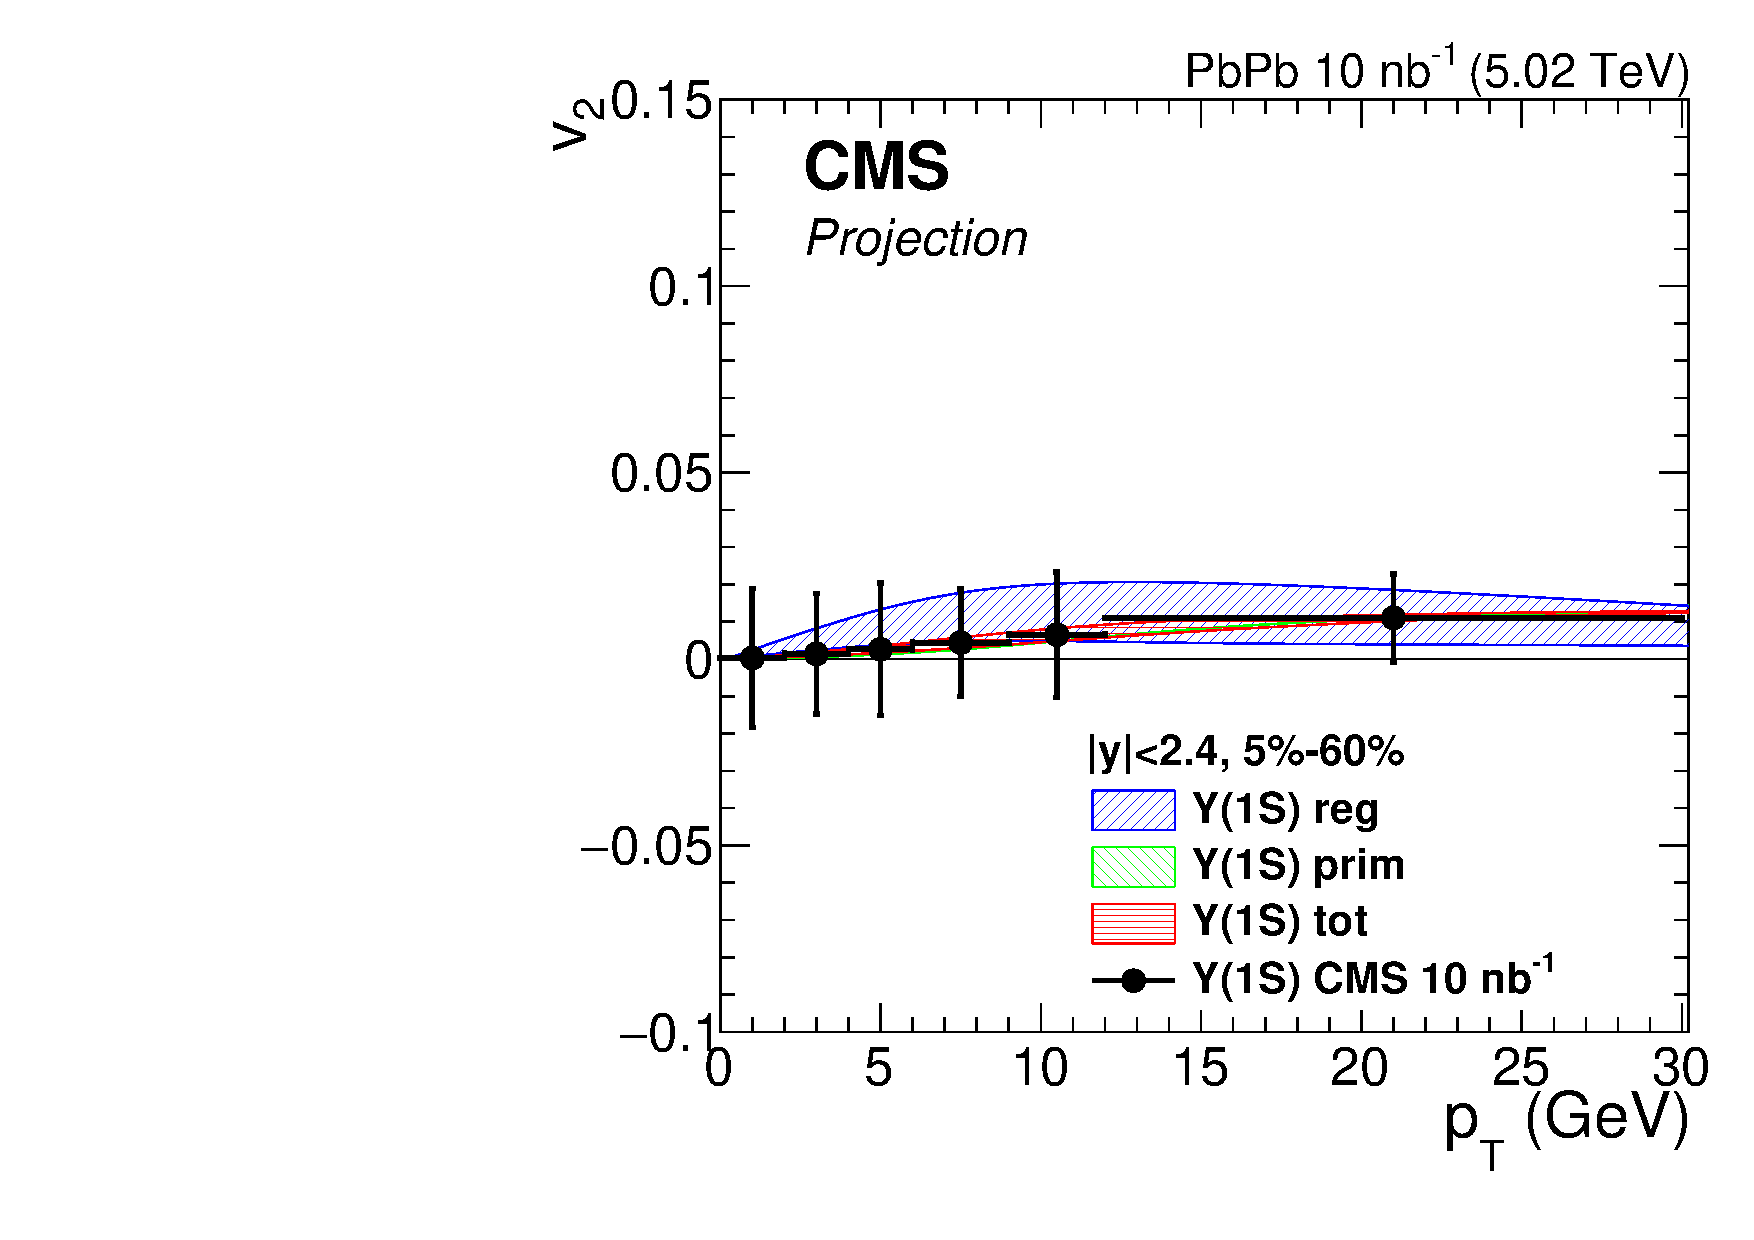
\includegraphics[width=0.3\textwidth]{\main/quarkonia/fig/cms/proj_Y1S_cent5-60.pdf}
 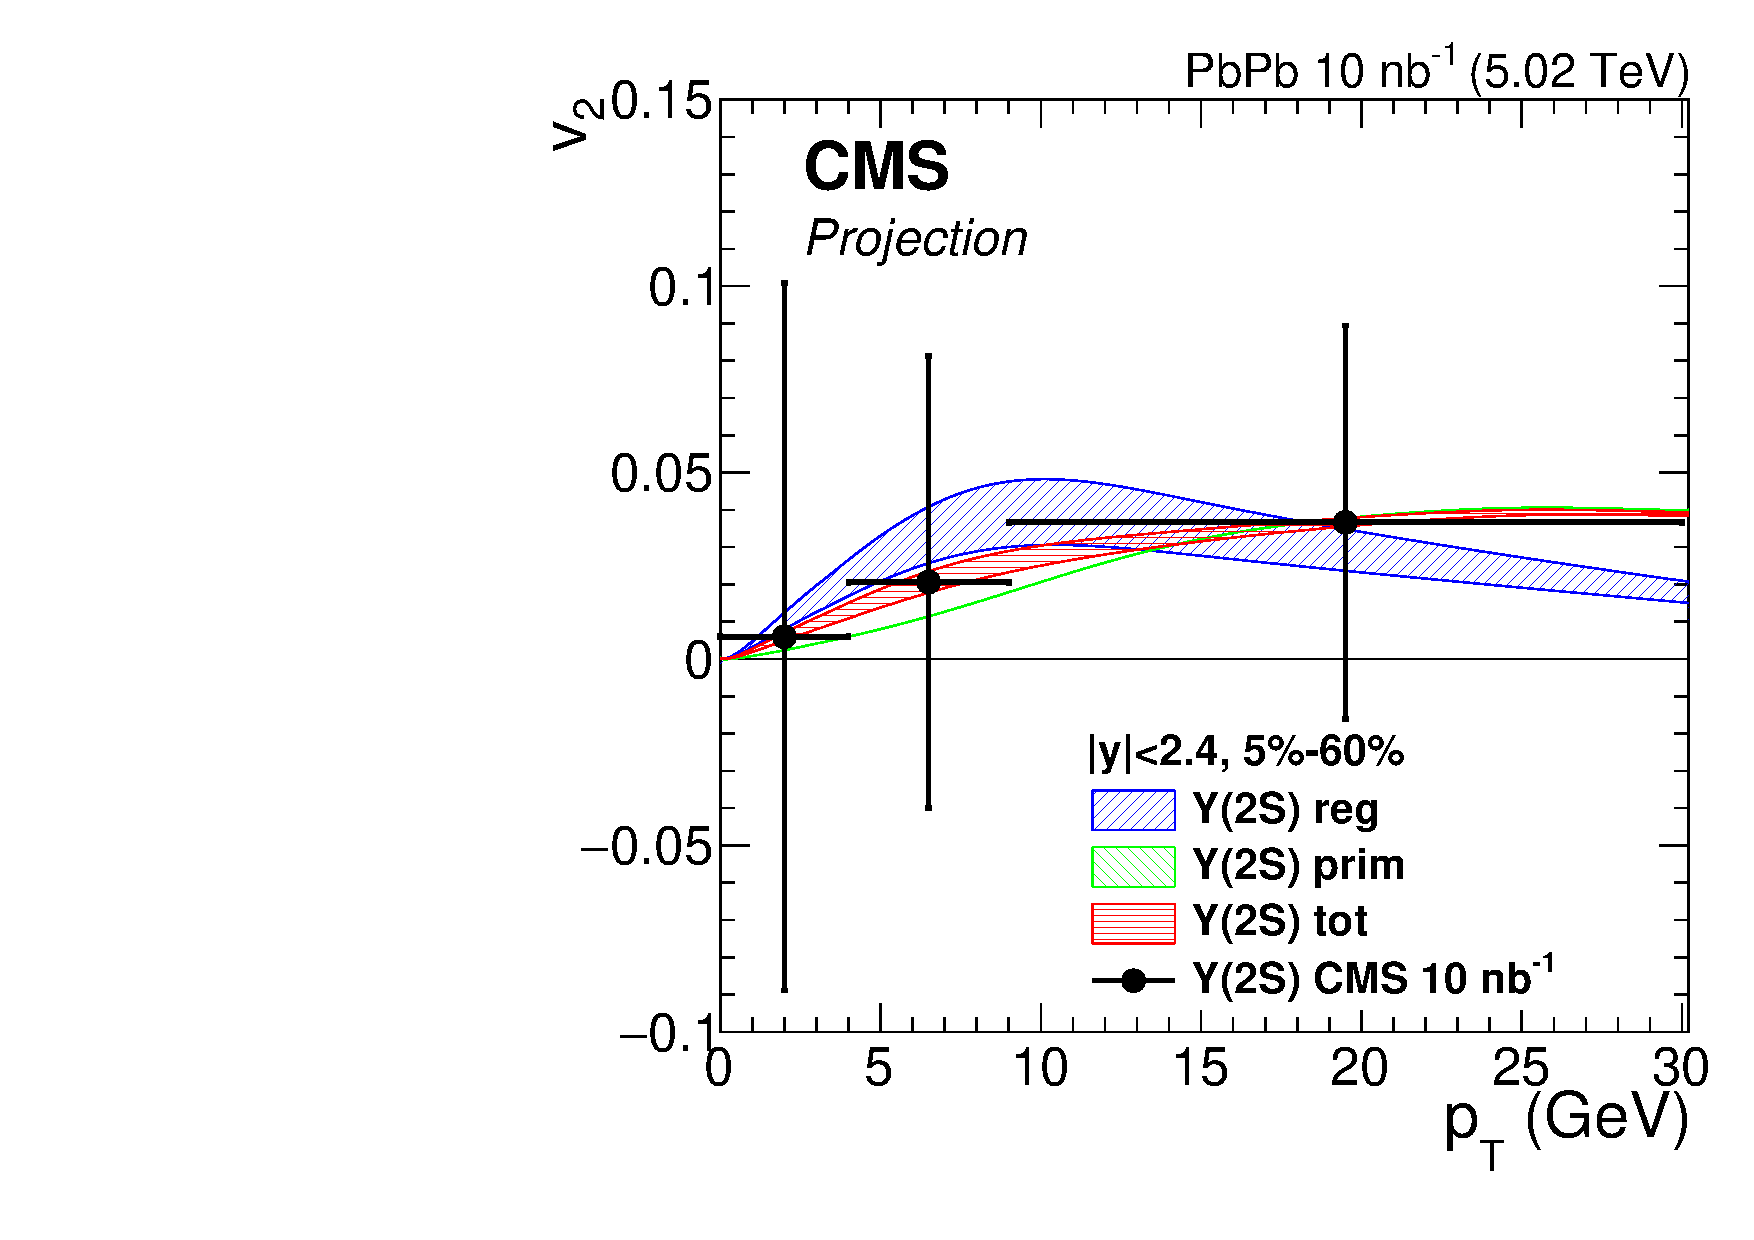
\includegraphics[width=0.3\textwidth]{\main/quarkonia/fig/cms/proj_Y2S_cent5-60.pdf}
 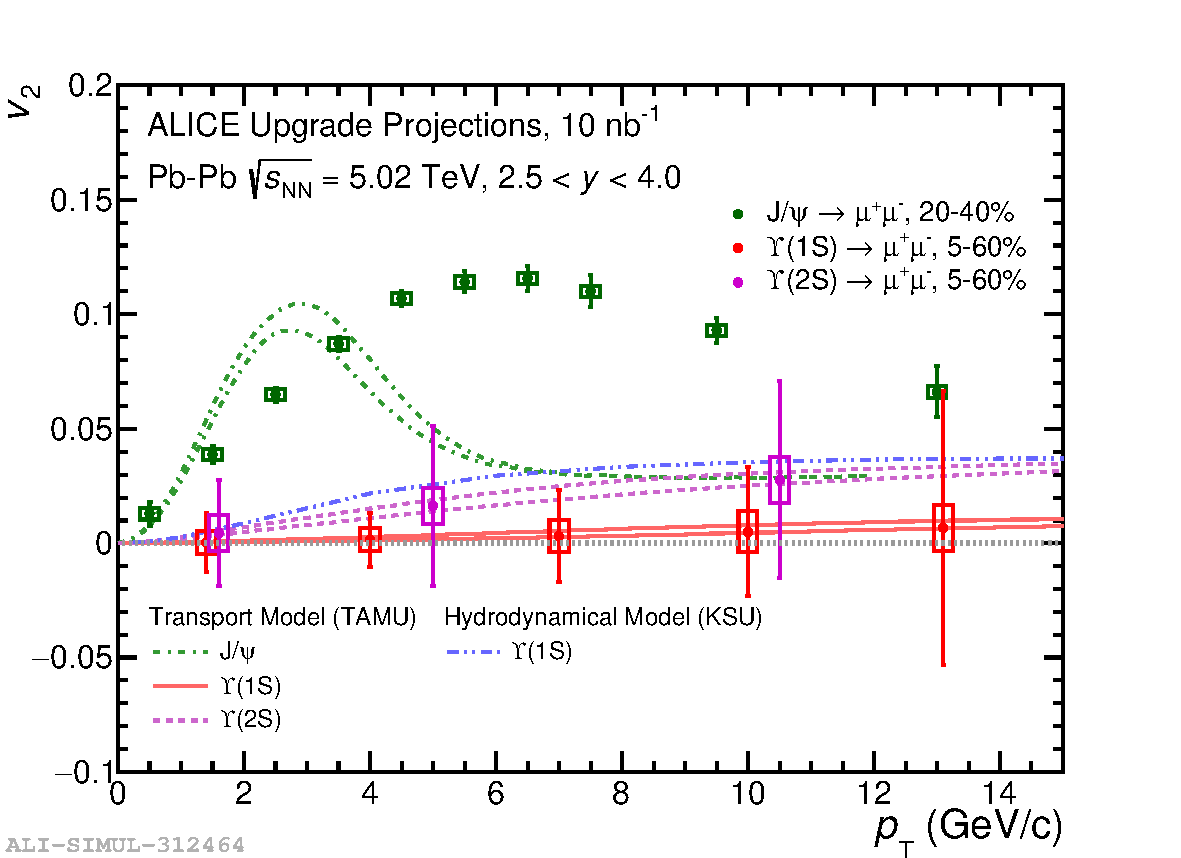
\includegraphics[width=0.38\textwidth]{\main/quarkonia/fig/alice/canvasFlow.pdf}
\end{center}

 \caption{$v_2$ projections for the CMS (left and centre) and ALICE (right) experiments (BOTH UNAPPROVED) for the \PGUP{1} and \PGUP{2} mesons, assuming the predictions from a transport model~\cite{Du:2017qkv}.}
 \label{fig:upsi_v2}
\end{figure}

% Discuss v2 
If we come back to the matter of regeneration, much can be learnt about it by a measurement of the elliptic flow of \PGUP{1} mesons~\cite{Das:2018xel}, 
unmeasured to date in any collision system. 
A parallel can be
drawn with that of \PJgy, which is still not properly described by models. This observable requires a more detailed implementation of the dynamics of the interactions between the 
quarkonium and the medium: thermalisation of the heavy quarks, time dependence of regeneration, path length dependence of energy loss, as well as initial geometry fluctuations and 
elastic rescattering of the quarkonia in the medium. Thus, collective flow brings complementary information to the \raa, and its measurement can help disentangle some
effects. In the case of \PGUP{1} mesons, a small $v_2$ (order of 1--2\%) is expected~\cite{Du:2017qkv,Yao:2018zrg}, as can be seen in Fig.~\ref{fig:upsi_v2},
essentially because the ground state is formed early in the fireball evolution, at a time when 
anisotropies are limited. For the same reason, the elliptic flow of \PGUP{2} could be a factor 2 or more higher~\cite{Du:2017qkv}, both from the regenerated and primordial
components. For both states, projections show that experimental precision may not be enough for a significant $v_2$ measurement, assuming $v_2$ values as in Ref.~\cite{Du:2017qkv}. For this reason,
combining results between the different LHC experiments would be beneficial to reach a better sensitivity.

% few sentences about spectra (instead of raa): measure them, more direct comparison to models, already measured now, etc
While we have focused on the \raa and $v_2$ in this section, bottomonium production can be studied using other observables. For instance, fully corrected yields or cross sections
in \PbPb can be studied, without making the ratio to a \pp measurement in a \raa. Such a measurement, already reported in some of the available experimental results~\cite{Sirunyan:2018nsz},
can directly be compared to a production model. 

% Also a figure on the prospects for the $B_c$ meson?

\clearpage

\subsection{Quarkonia in \pPb and \pp collisions (Main contributor: J.P. Lansberg)}

[{\it Be careful to avoid duplicate with the "small systems" section}]


\subsubsection{\pPb collisions}
 Quarkonium-production studies in high-energy \pPb collisions are usually carried out to measure how much specific nuclear effects, those which do {\it not} result from the creation of a deconfined state of matter, can alter the quarkonium yields. They should indeed be accounted for in the interpretation of  \PbPb collisions results. They are also interesting on their own as they provide one with means to probe the modification of the gluon densities in the nuclei, the interaction between such pure heavy-quark bound states and light hadrons, or phenomena such as the coherent medium-induced energy loss off these quark pairs.
 
 Usually, one distinguishes the {\it initial} and {\it final}-states effects\footnote{although the energty loss can be seen as an interplay between these}. Yet, it is probably more instructive to separate out the effects which are believed to impact {\it all} the states of the charmonium or the bottomonium family with the {\it same} magnitude from those which are expected to affect much more the excited states. In principle, initial-state effects are of the first kind as the nature of the to-be produced quarkonium state is not yet fixed where the effects take place.  On the contrary, final-state effects can be sensitive to the properties of the produced quarkonium state and can thus be of the second kind.
 
However, in \pPb collisions at LHC energies, final-state interactions between the heavy-quark pair and the nuclear matter likely occur {\it before} the pair hadronises. This is due to the large boost between the nucleus and the pair -- and thus the quarkonium. At rest, a $c \bar c$ or $b\bar b$ pair takes 0.3--0.4\,fm to hadronise. Seen from the nucleus, at for instance $y^{\rm lab}_{\rm pair}-y_{\rm beam} \sim 7$ , it takes $\gamma=\cosh(7) \simeq 500$ times longer! As such, final-state interactions with the nucleus likely not discriminate ground and excited quarkonium states. Such an argument based on the existence of a large boost is nevertheless not applicable if one considers effects arising from the interactions between the pair and other particles {\it produced} by the \pPb collisions, not those contained in the Pb nucleus. The former are indeed not moving at the Pb projectile rapidity. In fact, some of these particles can have similar rapidities to the quarkonium one and can thus be considered as comoving with it.
 
The simultaneous study of open-heavy flavoured hadrons along with both ground and excited quarkonium states is meant to shed light of all these phenomena. Along the lines exposed above, one expects forward-quarkonium production in \pPb collisions (namely when the quarkonia flies in the direction of the proton) to be sensitive to low-$x$ phenomena like the gluon shadowing or saturation in the lead ion or to the so-called coherent energy loss. On the contrary, the backward production should be sensitive to the gluon antishadowing. Moreover, the scatterings of quarkonia with comoving particles occur more often backward than forward, due to the rapidity-asymmetric particle multiplicities, and more often as well with the larger and less tightly bound excited states. 
   
With a wide rapidity coverage spanning from quasi -5 to 5, the LHC data from the 4 experiments are unique as they allow one to probe much smaller $x$ values than at RHIC and a with larger reach in $\pT$. The higher CM system energy, the competitive luminosities and the resolution of the detectors also allow for more extensive studies of the bottomonium family. In fact, the probably most striking observation made during the RUN 1 was that of a relative suppression in \pPb collisions of the excited \PGUP{2},\PGUP{3} states compared to that of the \PGUP{1} observed by CMS~\cite{Chatrchyan:2013nza}, recently confirmed by ATLAS~\cite{Aaboud:2017cif}. Not only it was unforeseen but it casted doubts on the conventional interpretation of the same suppression pattern observed in \PbPb collisions~\cite{Chatrchyan:2012lxa}. Such a relative suppression was also observed in the charmonium sector~\cite{Abelev:2014zpa}.

As far as the suppression of the \PGUP{1} and \PJgy is concerned, they seem to follow the expectations based on the RHIC results with a strong forward suppression compatible with a strong shadowing -- of a compatible magnitude of that observed with HF data~\cite{Kusina:2017gkz}. We should however note that the same observation can be explained by the coherent energy loss~\cite{Arleo:2010rb}. More data, including that on \PGU and Drell-Yan-pair production, are clearly needed to disentangle both effects. More precision for \PGU and non prompt \PJgy is in general critically needed as the typical experimental uncertainties are still on the order of the expected effects. As a case in point, backward $y$ data are not yet precise enough to quantify the magnitude of the gluon antishadowing.  The reader is referred to section 11 for more details on the constraints brought in by quarkonium \pPb LHC data on nuclear PDF fits.

Recently, the measurement of \PJgy $v_2$ in \pPb collisions became available~\cite{Acharya:2017tfn,CMS:2018xac}. They seem to indicate a significant -- and completely unexpected -- flow which may question the overall interpretation of the quarkonium $R^{\rm \pPb}$ measurements. More precise data are therefore crucial including additional correlations measurements. 

More precise Run 3 \& 4 data can thus expediently advance such studies in 4 directions:  
\begin{itemize}
\item  \PGU and non-\PJgy  $R^{\pPb}$ differential in $y$;
\item  \PJgy $R^{\pPb}$ at higher \pT\, double differential distribution in \pT\ \& $y$ as well as $v_2$ measurements; 
\item $\psi(2S)$ and \PGUP{2},\PGUP{3} $R^{\rm \pPb}$ with possibly some $v_2$ analyses,
then $R^{\rm \pPb}$ for new states including  the  $\chi_c(nP)$ and $\chi_b(nP)$ and possibly the $\eta_c$;
\item new observables such as associated-production channels already studied in \pp collisions {\bf [I can add Refs if needed]}  .



\end{itemize}
In addition to conventional LHC collider data, one should not overlook the discriminating power of data which can be collected in the fixed-target mode~\cite{Brodsky:2012vg,Lansberg:2012kf}. Not only they correspond to completely different energy and (CM) rapidity ranges, but extremely competitive luminosities -- up to fb$^{-1}$ -- are easily reachable. This is far beyond anything which can be reached in the collider mode during Run 3 \& 4. The LHCb collaboration has paved the way for a full fixed-target program at the LHC with their SMOG luminosity monitor~\cite{FerroLuzzi:2005em} used as an internal (He, Ne, Ar) gas target. {\bf Fig. shows ...\cite{LHCb:2017qap}} It is now clear that corresponding studies to those suggested above are possible~\cite{Hadjidakis:2018ifr} with the LHCb and ALICE detectors with light technical adjustments. They would drastically expand the scope of current proton-nucleus quarkonium studies.


\begin{figure}[hbt!]
 \begin{center}
 ~\\
 theory curves here
\\
~\\
 \end{center}
 \caption{RpA vs pT for excited states: psi(2S), upsilon(2S,3S), chic(1P) (separately for negative and positive $y_{CM}$)}
\end{figure}

\begin{figure}
 \begin{center}
  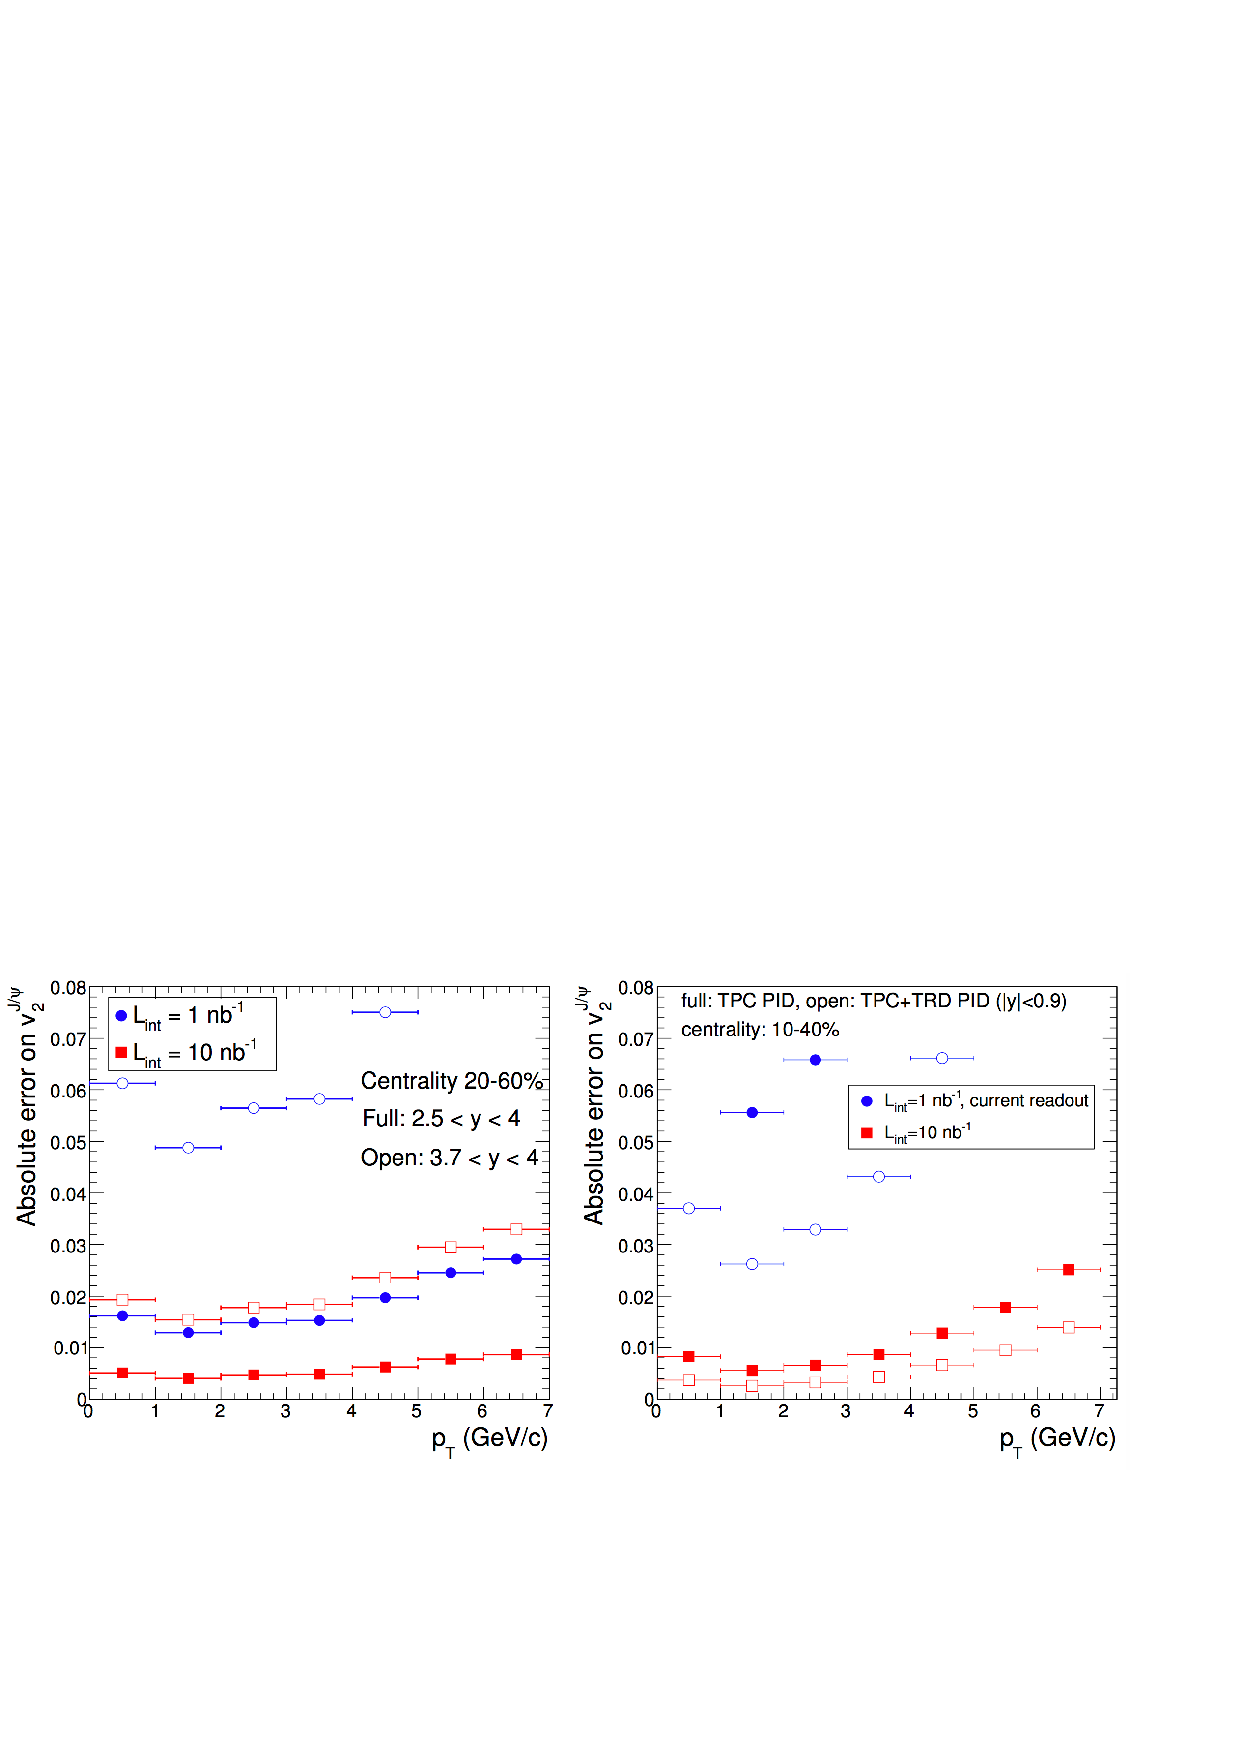
\includegraphics[width=0.32\textwidth]{\main/quarkonia/fig/alice/alice_jpsi_v2_projected.pdf}
  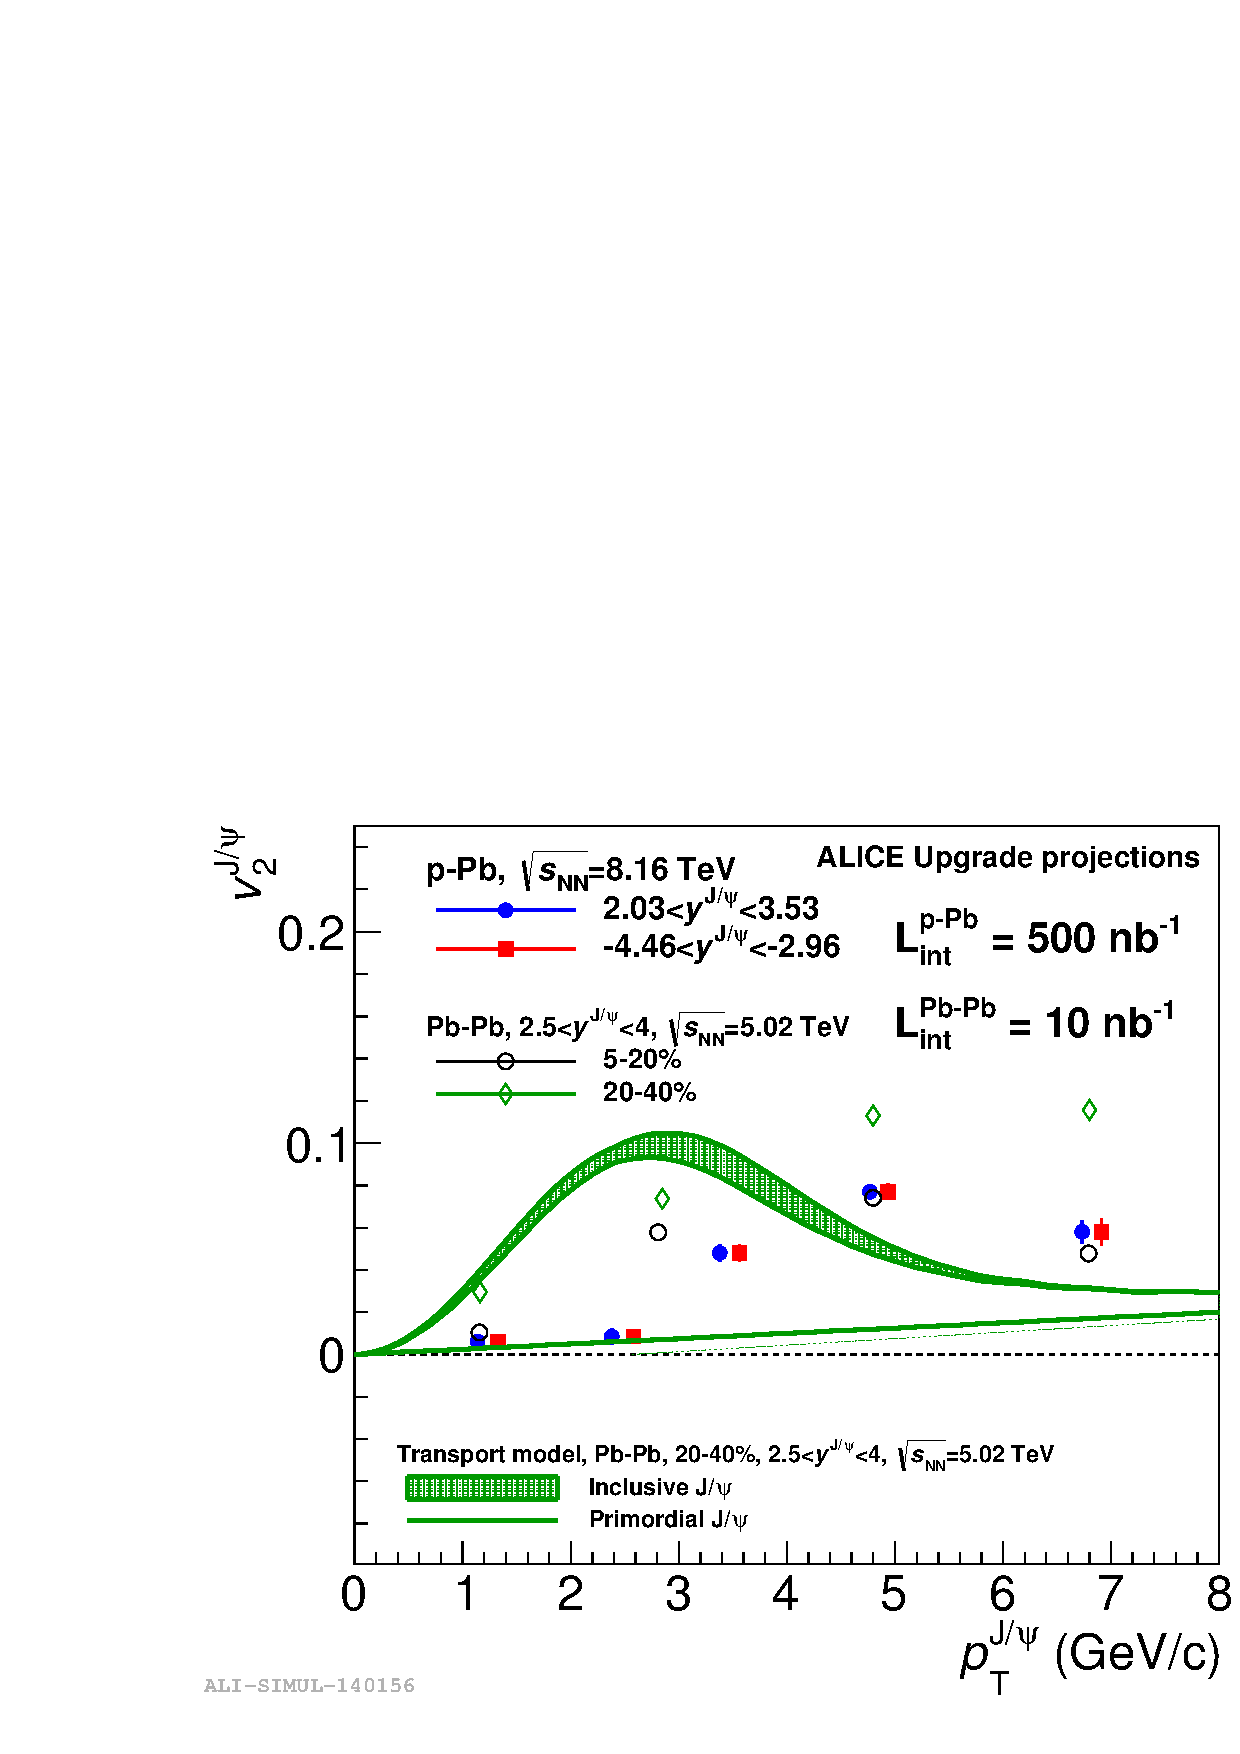
\includegraphics[width=0.32\textwidth]{\main/quarkonia/fig/alice/alice_jpsi_v2_projected2.pdf}
 \end{center}

 \caption{prompt J/psi v2 and v3 (separately for negative and positive $y_{CM}$)}
\end{figure}

\begin{figure}
 \begin{center}
  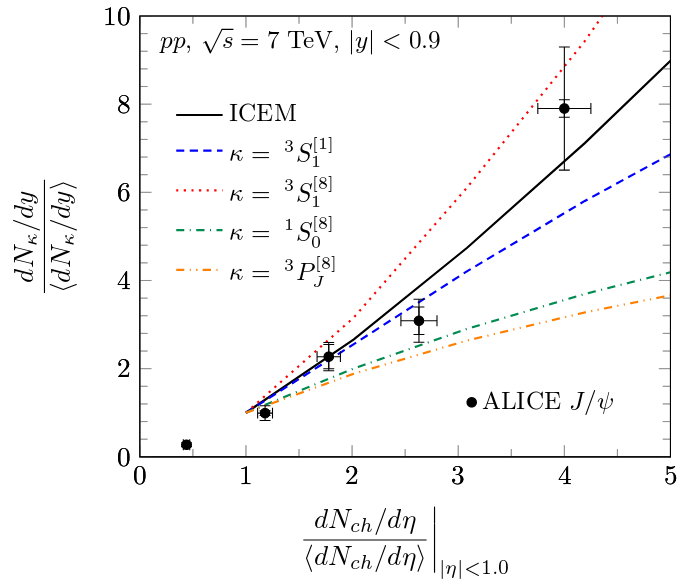
\includegraphics[width=0.5\textwidth]{\main/quarkonia/fig/theory/cgc_jpsi_nch.png}
 \end{center}

 \caption{prompt J/psi vs Nch (also in \pp)~\cite{Ma:2018bax}}
\end{figure}

\begin{figure}
 \begin{center}
 theory curves here
 \end{center}

 \caption{RpA vs pT for excited states: psi(2S), upsilon(2S,3S), chic(1P) (separately for negative and positive $y_{CM}$)}
\end{figure}

To be also discussed: SMOG results from LHCb.

\subsection*{Acknowledgement}
RR has been supported by the US National Science Foundation under
grant number PHY-1614484, and in part by the ExtreMe Matter Institute EMMI at 
the GSI Helmholtzzentrum f\"{u}r Schwerionenforschung (Darmstadt,Germany).

\end{document}
